\documentclass{vkr}
\usepackage[english, russian]{babel} % переносы
\usepackage{graphicx} % для вставки картинок
\graphicspath{{images/}} % путь к изображениям
\usepackage[hidelinks]{hyperref}
\AtBeginDocument{%
	\renewcommand{\theHtable}{\thesection.\arabic{table}}%
}
\usepackage{float} % определяет метод H для рисунка с переносом на следующую страницу, ели не помещается
\usepackage{pdflscape}
\addto{\captionsrussian}{\renewcommand{\refname}{СПИСОК ИСПОЛЬЗОВАННЫХ ИСТОЧНИКОВ}}
\usepackage{xltabular} % для вставки таблиц
\usepackage{makecell}
\usepackage{setspace}
\renewcommand\theadfont{} % шрифт в /thead
\usepackage{array} % для определения новых типов столбцов таблиц
\newcolumntype{T}{>{\centering\arraybackslash}X} % новый тип столбца T - автоматическая ширина столбца с выравниванием по центру
\newcolumntype{R}{>{\raggedleft\arraybackslash}X} % новый тип столбца R - автоматическая ширина столбца с выравниванием по правому краю
\newcolumntype{C}[1]{>{\centering\let\newline\\\arraybackslash\hspace{0pt}}m{#1}} % новый тип столбца C - фиксированная ширина столбца с выравниванием по центру
\newcolumntype{r}[1]{>{\raggedleft\arraybackslash}p{#1}} % новый тип столбца r - фиксированная ширина столбца с выравниванием по правому краю
\newcolumntype{P}[1]{>{\raggedright\arraybackslash\hspace{0pt}}p{#1}} % перенос длинных имён в ячейках таблиц
\usepackage{xurl}
\urlstyle{same}
\newcommand{\codeid}[1]{\nolinkurl{#1}} % идентификаторы кода с переносом по символам
\newcommand{\centrow}{\centering\arraybackslash} % командой \centrow можно центрировать одну ячейку (заголовок) в столбце типа X или p, оставив в оcтальных ячейках другой тип выравнивания
\newcommand{\finishhead}{\endhead\hline\endlastfoot}
\newcommand{\continuecaption}[1]{\captionsetup{labelformat=empty} \caption[]{#1}\\ \hline }
\usepackage{etoolbox}
\AtBeginEnvironment{xltabular}{%
	\refstepcounter{tablecnt}%
}

\usepackage[tableposition=top]{caption} % подпись таблицы вверху
\captionsetup{strut=off}
\setlength{\intextsep}{0pt} % Vertical space above & below [h] floats
\setlength{\textfloatsep}{0pt} % Vertical space below (above) [t] ([b]) floats
\DeclareCaptionLabelFormat{gostfigure}{Рисунок #2} %подпись рисунка
\DeclareCaptionLabelFormat{gosttable}{Таблица #2} %подпись таблицы
\DeclareCaptionLabelSeparator{gost}{~--~} %разделитель в рисунках и таблицах
\captionsetup{labelsep=gost}
\captionsetup[figure]{aboveskip=10pt,belowskip=4mm,justification=centering,labelformat=gostfigure} % настройка подписи рисунка
\captionsetup[table]{font={stretch=1.41},skip=0pt,belowskip=0pt,aboveskip=8.5pt,singlelinecheck=off,labelformat=gosttable} % настройка подписи таблицы

\setlength{\LTpre}{8mm} % отступ сверху таблицы
\setlength{\LTpost}{6mm} % отступ снизу таблицы

\usepackage{enumitem}
\setlist{nolistsep,wide=\parindent,itemindent=*} % отступы вокруг списков, выравнивание с учетом разделителя

\usepackage{color} %% это для отображения цвета в коде
\usepackage{listings} %% листинги кода
\setmonofont[Scale=0.7]{Verdana} % моноширный шрифт для листинга

\definecolor{codegreen}{rgb}{0,0.6,0}
\definecolor{codegray}{rgb}{0.5,0.5,0.5}
\definecolor{codepurple}{rgb}{0.58,0,0.82}

\lstset{ %
language=C,                 % выбор языка для подсветки (здесь это С)
numbers=left,               % где поставить нумерацию строк (слева\справа)
numberstyle=\tiny,           % размер шрифта для номеров строк
stepnumber=1,                   % размер шага между двумя номерами строк
numbersep=5pt,                % как далеко отстоят номера строк от подсвечиваемого кода
commentstyle=\color{codegreen},
keywordstyle=\color{magenta},
numberstyle=\tiny\color{codegray},
stringstyle=\color{codepurple},
basicstyle=\linespread{0.95}\ttfamily,
backgroundcolor=\color{white}, % цвет фона подсветки - используем \usepackage{color}
showspaces=false,            % показывать или нет пробелы специальными отступами
showstringspaces=false,      % показывать или нет пробелы в строках
showtabs=false,             % показывать или нет табуляцию в строках
frame=single,              % рисовать рамку вокруг кода
tabsize=2,                 % размер табуляции по умолчанию равен 2 пробелам
captionpos=t,              % позиция заголовка вверху [t] или внизу [b] 
breaklines=true,           % автоматически переносить строки (да\нет)
breakatwhitespace=false, % переносить строки только если есть пробел
escapeinside={\%*}{*)}   % если нужно добавить комментарии в коде
}

\makeatletter % чтобы допускались русские комментарии в листингах
\lst@InputCatcodes
\def\lst@DefEC{%
 \lst@CCECUse \lst@ProcessLetter
  ^^80^^81^^82^^83^^84^^85^^86^^87^^88^^89^^8a^^8b^^8c^^8d^^8e^^8f%
  ^^90^^91^^92^^93^^94^^95^^96^^97^^98^^99^^9a^^9b^^9c^^9d^^9e^^9f%
  ^^a0^^a1^^a2^^a3^^a4^^a5^^a6^^a7^^a8^^a9^^aa^^ab^^ac^^ad^^ae^^af%
  ^^b0^^b1^^b2^^b3^^b4^^b5^^b6^^b7^^b8^^b9^^ba^^bb^^bc^^bd^^be^^bf%
  ^^c0^^c1^^c2^^c3^^c4^^c5^^c6^^c7^^c8^^c9^^ca^^cb^^cc^^cd^^ce^^cf%
  ^^d0^^d1^^d2^^d3^^d4^^d5^^d6^^d7^^d8^^d9^^da^^db^^dc^^dd^^de^^df%
  ^^e0^^e1^^e2^^e3^^e4^^e5^^e6^^e7^^e8^^e9^^ea^^eb^^ec^^ed^^ee^^ef%
  ^^f0^^f1^^f2^^f3^^f4^^f5^^f6^^f7^^f8^^f9^^fa^^fb^^fc^^fd^^fe^^ff%
  ^^^^20ac^^^^0153^^^^0152%
  % Basic Cyrillic alphabet coverage
  ^^^^0410^^^^0411^^^^0412^^^^0413^^^^0414^^^^0415^^^^0416^^^^0417%
  ^^^^0418^^^^0419^^^^041a^^^^041b^^^^041c^^^^041d^^^^041e^^^^041f%
  ^^^^0420^^^^0421^^^^0422^^^^0423^^^^0424^^^^0425^^^^0426^^^^0427%
  ^^^^0428^^^^0429^^^^042a^^^^042b^^^^042c^^^^042d^^^^042e^^^^042f%
  ^^^^0430^^^^0431^^^^0432^^^^0433^^^^0434^^^^0435^^^^0436^^^^0437%
  ^^^^0438^^^^0439^^^^043a^^^^043b^^^^043c^^^^043d^^^^043e^^^^043f%
  ^^^^0440^^^^0441^^^^0442^^^^0443^^^^0444^^^^0445^^^^0446^^^^0447%
  ^^^^0448^^^^0449^^^^044a^^^^044b^^^^044c^^^^044d^^^^044e^^^^044f%
  ^^^^0401^^^^0451%
  %%%
  ^^00}
\lst@RestoreCatcodes
\makeatother


% Режим шаблона (должен быть включен один из трех)
\ВКРtrue
%\Практикаtrue
%\Курсоваяtrue

\newcommand{\Дисциплина}{<<Проектирование и архитектура программных систем>>} % для курсовой
\newcommand{\КодСпециальности}{09.03.04} % Курсовая
\newcommand{\Специальность}{Программная инженерия} % Курсовая
\newcommand{\Тема}{Бизнес-проект <<Приложение для составления}
\newcommand{\ТемаВтораяСтрока}{тренировочного плана и отслеживания прогресса>>. Клиентская часть}
\newcommand{\ГдеПроводитсяПрактика}{АНО ДПО «УНЦИЯ»} % для практики
\newcommand{\РуководительПрактПредпр}{Лескова И. В.} % для практики
\newcommand{\ДолжнРуководительПрактПредпр}{президент} % для практики
\newcommand{\РуководительПрактУнивер}{Чаплыгин А. А.} % для практики
\newcommand{\ДолжнРуководительПрактУнивер}{к.\,т.\,н., доцент} % для практики
\newcommand{\Автор}{А.\,Г. Бантьев}
\newcommand{\АвторРод}{Бантьев А.\,Г.}
\newcommand{\АвторПолностьюРод}{Бантьева Артема Геннадиевича} % для практики
\newcommand{\Шифр}{22-06-0171}
\newcommand{\Курс}{4 } % для практики
\newcommand{\Группа}{ПО-21б}
\newcommand{\Руководитель}{И.\,Н. Ефремова} % для ВКР и курсовой
\newcommand{\Нормоконтроль}{А. А. Чаплыгин} % для ВКР
\newcommand{\ЗавКаф}{А. В. Малышев} % для ВКР
\newcommand{\ДатаПриказа}{«03» апреля 2026~г.} % для ВКР
\newcommand{\НомерПриказа}{1584-с} % для ВКР
\newcommand{\СрокПредоставления}{«9» июня 2026~г.} % для ВКР, курсового

\begin{document}
\maketitle
\ifПрактика{}\else{
   \newpage
\begin{center}
\large\textbf{Минобрнауки России}

\large\textbf{Юго-Западный государственный университет}
\vskip 1em
\normalsize{Кафедра программной инженерии}
\vskip 1em
\ifВКР{
        \begin{flushright}
        \begin{tabular}{p{.4\textwidth}}
        \centrow УТВЕРЖДАЮ: \\
        \centrow Заведующий кафедрой \\
        \hrulefill \\
        \setarstrut{\footnotesize}
        \centrow\footnotesize{(подпись, инициалы, фамилия)}\\
        \restorearstrut
        «\underline{\hspace{1cm}}»
        \underline{\hspace{3cm}}
        20\underline{\hspace{1cm}} г.\\
        \end{tabular}
        \end{flushright}
        }\fi
\end{center}
\vspace{1em}
  \begin{center}
  \large
\ifВКР{
ЗАДАНИЕ НА ВЫПУСКНУЮ КВАЛИФИКАЦИОННУЮ РАБОТУ
  ПО ПРОГРАММЕ БАКАЛАВРИАТА}
  \else
ЗАДАНИЕ НА КУРСОВУЮ РАБОТУ (ПРОЕКТ)
\fi
\normalsize
  \end{center}
\vspace{1em}
{\parindent0pt
  Студента \АвторРод, шифр\ \Шифр, группа \Группа
  
1. Тема «\Тема\ \ТемаВтораяСтрока»
\ifВКР{
утверждена приказом ректора ЮЗГУ от \ДатаПриказа\ № \НомерПриказа
}\fi.

2. Срок предоставления работы к защите \СрокПредоставления

3. Исходные данные для создания программной системы:

3.1. Перечень решаемых задач:}

\renewcommand\labelenumi{\theenumi)}

\begin{enumerate}
\item изучение предметной области индивидуальных тренировок и существующих цифровых решений в сфере фитнеса;
\item проектирование клиент-серверной архитектуры веб-приложения с выделением клиентской подсистемы;
\item проектирование структуры одностраничного интерфейса, навигации и модулей клиентского приложения;
\item реализация экранов регистрации, входа и управления профилем пользователя;
\item реализация клиентских модулей планирования тренировок, учёта занятий и визуализации прогресса;
\item реализация клиентских модулей питания, психологической поддержки, аватара и социальной ленты;
\item организация локального хранения состояния и синхронизации данных с REST API серверной части;
\item тестирование клиентского приложения в браузере и проверка основных пользовательских сценариев.
\end{enumerate}

{\parindent0pt
  3.2. Входные данные и требуемые результаты для программы:}

\begin{enumerate}
\item Входными данными для клиентской подсистемы являются: действия пользователя в браузере (ввод в формы, переключение разделов, выбор упражнений и продуктов), ответы REST API серверной части в формате JSON, справочные данные приложения (каталог упражнений, шаблоны программ, локальные JSON-файлы).
\item Выходными данными для клиентской подсистемы являются: отображение интерфейса приложения, формирование HTTP-запросов к API, сохранение клиентского состояния в \texttt{localStorage}, визуализация прогресса (графики, календарь, аналитика нагрузки), обеспечение работоспособности модулей тренировок, питания, поддержки, аватара и социальной ленты.
\end{enumerate}

{\parindent0pt

  4. Содержание работы (по разделам):
  
  4.1. Введение.
  
  4.2. Анализ предметной области.
  
4.3. Техническое задание: основание для разработки, назначение разработки,
требования к программной системе, требования к оформлению документации.

4.4. Технический проект: общие сведения о программной системе, обоснование выбора технологий, проектирование архитектуры клиентского приложения, проектирование пользовательского интерфейса программной системы.

4.5. Рабочий проект: спецификация клиентских модулей и компонентов, тестирование программной системы, сборка и проверка клиентского приложения.

4.6. Заключение.

4.7. Список использованных источников.

5. Перечень графического материала:

\списокПлакатов

\vskip 2em
\begin{tabular}{p{6.8cm}C{3.8cm}C{4.8cm}}
Руководитель \ifВКР{ВКР}\else работы (проекта) \fi & \lhrulefill{\fill} & \fillcenter\Руководитель\\
\setarstrut{\footnotesize}
& \footnotesize{(подпись, дата)} & \footnotesize{(инициалы, фамилия)}\\
\restorearstrut
Задание принял к исполнению & \lhrulefill{\fill} & \fillcenter\Автор\\
\setarstrut{\footnotesize}
& \footnotesize{(подпись, дата)} & \footnotesize{(инициалы, фамилия)}\\
\restorearstrut
\end{tabular}
}

\renewcommand\labelenumi{\theenumi.}

   \abstract{РЕФЕРАТ}

Объем работы равен \formbytotal{lastpage}{страниц}{е}{ам}{ам}. Работа содержит \formbytotal{figurecnt}{иллюстраци}{ю}{и}{й}, \formbytotal{tablecnt}{таблиц}{у}{ы}{}, \arabic{bibcount} библиографических источников и \formbytotal{числоПлакатов}{лист}{}{а}{ов} графического материала. Количество приложений – 2. Графический материал представлен в приложении А. Фрагменты исходного кода представлены в приложении Б.

Перечень ключевых слов: фитнес, программно-информационная система, клиент, web-приложение, одностраничное приложение, тренировочный план, прогресс, пользователь, интерфейс, профиль, тренировки, питание, социальная лента, DOM, JavaScript, HTML, CSS, REST API, модуль, браузер.

Объектом разработки является клиентская часть программно-информационной системы <<Fitness Life>>, обеспечивающая регистрацию и вход пользователей, работу с тренировочными планами и дневником питания, визуализацию прогресса, взаимодействие с модулями поддержки, аватара и социальной ленты, а также обмен данными с серверной подсистемой через REST API.

Целью выпускной квалификационной работы является создание клиентской подсистемы веб-приложения, обеспечивающей планирование тренировок, отслеживание прогресса, удобный пользовательский интерфейс и синхронизацию персональных данных с серверной частью.

В процессе разработки клиентской части системы была выделена клиент-серверная архитектура, спроектирована модульная структура одностраничного приложения, реализованы экраны аутентификации и профиля, клиентские модули тренировок, питания, психологической поддержки, аватара и социальной ленты, а также механизмы локального хранения состояния и обращения к REST API.

При разработке клиентской части использовались HTML, CSS, JavaScript (модули *.module.js), библиотека Chart.js, Web Storage API (localStorage).

\selectlanguage{english}
\abstract{ABSTRACT}
  
The volume of work is \formbytotal{lastpage}{page}{}{s}{s}. The work contains \formbytotal{figurecnt}{illustration}{}{s}{s}, \formbytotal{tablecnt}{table}{}{s}{s}, \arabic{bibcount} bibliographic sources and \formbytotal{числоПлакатов}{sheet}{}{s}{s} of graphic material. The number of applications is 2. Graphic material is presented in annex A. Source code fragments are presented in annex B.

List of keywords: fitness, information system, client, web application, single-page application, workout plan, progress, user, interface, profile, training, nutrition, social feed, DOM, JavaScript, HTML, CSS, REST API, module, browser.

The object of development is the client part of the Fitness Life information system providing user registration and login, workout planning and nutrition diary, progress visualization, support and avatar modules, social feed interaction, and data exchange with the server subsystem via a REST API.

The purpose of the thesis is to create a client subsystem of a web application that supports workout planning, progress tracking, a convenient user interface, and synchronization of personal data with the server part.

During the development of the client part, a client-server architecture was defined, a modular single-page application structure was designed, authentication and profile screens were implemented, client modules for training, nutrition, psychological support, avatar, and social feed were developed, along with local state storage and REST API access mechanisms.

HTML, CSS, JavaScript (*.module.js modules), the Chart.js library, and the Web Storage API (localStorage) were used in the development of the client part.
\selectlanguage{russian}
}\fi
\tableofcontents
\section*{ОБОЗНАЧЕНИЯ И СОКРАЩЕНИЯ}

API (Application Programming Interface) -- программный интерфейс приложения.

CSS (Cascading Style Sheets) -- каскадные таблицы стилей.

DOM (Document Object Model) -- объектная модель документа, используемая браузером для представления HTML-страницы.

HTML (HyperText Markup Language) -- язык гипертекстовой разметки.

HTTP(S) -- протокол передачи гипертекста.

JS (JavaScript) -- язык программирования, используемый для реализации интерактивности веб-страниц.

JSON (JavaScript Object Notation) -- текстовый формат обмена данными.

SPA (Single Page Application) -- одностраничное веб-приложение.

UI (User Interface) -- пользовательский интерфейс.

UX (User Experience) -- пользовательский опыт.

ИС -- информационная система.

ПО -- программное обеспечение.

ТЗ -- техническое задание.

ТП -- технический проект.

UML (Unified Modelling Language) -- язык графического описания для объектного моделирования в области разработки программного обеспечения.

\ifВКР{\newpage
\section*{РЕЗЮМЕ СТАРТАП-ПРОЕКТА}
\addcontentsline{toc}{section}{РЕЗЮМЕ СТАРТАП-ПРОЕКТА}


Название: <<Бизнес-проект <<Приложение для составления тренировочного плана и отслеживания прогресса.>> Клиентская часть>>. Проект представляет собой программно-информационную систему, предназначенную для организации самостоятельных занятий физической культурой: составления индивидуального плана нагрузки, учёта выполненных упражнений, контроля питания и обмена результатами между пользователями. Система обеспечивает регистрацию и вход в личный кабинет, ведение профиля с учётом целей и антропометрических данных, формирование и хранение тренировочных планов, фиксацию подходов и анализ прогресса, ведение дневника питания, работу социальной ленты, а также синхронизацию данных между браузером пользователя и сервером с защитой персональной информации.

Ключевые возможности системы включают:
\begin{enumerate}
	\item Составление и редактирование индивидуальных планов тренировок с учётом целей, уровня подготовки и предпочтений пользователя.
	
	\item Ведение журнала выполненных упражнений с фиксацией повторений, рабочего веса и нагрузки по группам мышц, а также наглядное отображение динамики прогресса и сводной статистики.
	
	\item Учёт питания и пользовательских настроек (цели по калориям и макронутриентам, собственные продукты) в едином веб-интерфейсе.
	
	\item Социальную ленту: публикации о тренировках и питании, комментарии, лайки и реакции для поддержания мотивации и обмена опытом.
	
	\item Интуитивно понятный и адаптивный графический интерфейс веб-клиента, поддерживающий работу на различных устройствах без установки отдельного мобильного приложения.
\end{enumerate}

Созданная система оптимизирует процесс самостоятельных тренировок, повышая наглядность контроля нагрузки и прогресса и позволяя пользователю объединить планирование занятий, учёт питания и социальное взаимодействие без переключения между несколькими узкоспециализированными сервисами.

\emph{Актуальность} проекта обусловлена ростом интереса к здоровому образу жизни и цифровым инструментам самоконтроля. Большинство популярных решений закрывают лишь отдельные задачи -- учёт силовых тренировок, дневник питания или социальную мотивацию -- и часто требуют подписки либо привязаны к конкретной платформе. Пользователю, занимающемуся без постоянного тренера, необходим доступный веб-сервис, который помогает организовать занятия, видеть результат и сохранять данные при работе с разных устройств, что снижает затраты времени на подбор разрозненных приложений.

\emph{Целью} разработки является создание программно-информационной системы <<Fitness Life>>, способной обеспечить:
\begin{itemize}
	\item персональное планирование тренировок и учёт выполненных занятий;
	
	\item отслеживание прогресса и наглядную аналитику физической нагрузки;
	
	\item ведение дневника питания в составе единого приложения;
	
	\item социальное взаимодействие пользователей для поддержания мотивации;
	
	\item надёжное хранение данных и доступ к личному кабинету с различных устройств через браузер.
\end{itemize}

\emph{Отличительные особенности} разработанной системы по сравнению с существующими решениями:
\begin{enumerate}
	\item Современный и интуитивно понятный интерфейс, адаптированный под сценарии планирования тренировок, учёта питания и работы с лентой.
	
	\item Объединение тренировочного плана, журнала занятий, учёта питания и социальной ленты в одном web-приложении.
	
	\item Гибкая настройка профиля и целей пользователя, облачная синхронизация данных между сеансами работы и устройствами.
	
	\item Возможность масштабирования и дальнейшей интеграции с мобильными платформами, носимыми устройствами и внешними фитнес-сервисами.
\end{enumerate}

В системе реализованы задачи по отображению экранов регистрации и входа, ведению профиля, формированию и хранению тренировочных планов на клиенте, фиксации выполненных упражнений и визуализации статистики прогресса, учёту питания, работе социальной ленты и синхронизации данных браузера с REST API серверной части, а также обеспечению модульной структуры клиентского приложения с использованием современных веб-технологий (HTML, CSS, JavaScript, Chart.js, localStorage).

Идея создания проекта возникла в 2025 году на фоне возросшего спроса на доступные цифровые инструменты для самостоятельных тренировок с облачным хранением прогресса, а разработка была начата в начале 2026 года. Завершение проекта планируется к середине 2026 года.

\emph{Бизнес-цели:}
\begin{enumerate}
	\item Расширение функциональных возможностей за счёт интеграции с трекерами активности, каталогами упражнений и внешними сервисами здоровья.
	
	\item Масштабирование системы для роста пользовательской базы с учётом различных целей занятий (силовые тренировки, похудение, поддержание формы).
	
	\item Добавление дополнительных функций: напоминания о тренировках, визуализация серий занятий, расширенные шаблоны программ и настройка интерфейса для повышения вовлечённости.
	
	\item Повышение регулярности занятий и удержание аудитории за счёт наглядного прогресса, социальной поддержки и модели freemium (базовый функционал бесплатно, расширенная аналитика -- по подписке).
\end{enumerate}
}\fi
\ifПрактика{}\else{\section*{ВВЕДЕНИЕ}
\addcontentsline{toc}{section}{ВВЕДЕНИЕ}

Рост популярности здорового образа жизни и самостоятельных занятий физической культурой сопровождается активным развитием цифровых сервисов: тренировочных дневников, трекеров активности, приложений учёта питания и социальных платформ для обмена результатами. Для пользователя, который планирует нагрузку без постоянного присутствия тренера, критичны не только справочные материалы об упражнениях, но и возможность формировать индивидуальный план, фиксировать выполнение, анализировать динамику и сохранять данные при работе с разных устройств. Эти требования естественно приводят к архитектуре <<клиент -- сервер -- база данных>>, в которой серверная часть обеспечивает аутентификацию, целостность персональной информации и единый контур обмена данными между клиентами, а клиентская часть отвечает за представление информации, ввод данных пользователем и выполнение сценариев работы в браузере.

Коммерческие решения на рынке, как правило, закрывают лишь отдельные аспекты задачи: одни продукты ориентированы на учёт силовых тренировок, другие -- на калорийность рациона, третьи -- на социальную мотивацию или экосистему носимых устройств. Объединение планирования тренировок, питания, профиля пользователя и социальной активности в одной системе при сохранении веб-доступа через браузер остаётся востребованной учебной и прикладной постановкой. В рамках настоящей выпускной квалификационной работы разрабатывается программно-информационная система <<Fitness Life>> -- бизнес-проект стартап-команды, в котором инженерный вклад автора сосредоточен на клиентской подсистеме: проектировании одностраничного интерфейса, организации модулей браузерного приложения, визуализации прогресса и взаимодействия с REST API серверной части.

Система <<Fitness Life>> реализуется как клиент-серверное веб-приложение. Серверная подсистема (разрабатывается напарником по проекту) построена на стеке Node.js и Express и взаимодействует с реляционной СУБД PostgreSQL: она принимает HTTP-запросы, проверяет учётные данные, выдаёт и проверяет JWT, хранит профили пользователей, синхронизируемое пользовательское хранилище ключ -- значение и данные социальной ленты. Клиентская подсистема представляет собой одностраничное приложение (SPA), загружаемое в браузере: HTML-разметка задаёт каркас экранов, CSS -- визуальное оформление и адаптивность, JavaScript -- интерактивную логику. После входа пользователь работает с единой оболочкой приложения и переключает разделы (тренировки, питание, социальная лента, поддержка, аватар, профиль) без полной перезагрузки страницы.

Связь клиента и сервера организована через REST API по протоколу HTTP(S) в формате JSON. Модуль auth.js выполняет регистрацию и вход, сохраняет токен и сведения о пользователе, при успешной аутентификации подгружает данные с сервера и синхронизирует ключи localStorage с таблицей user\_storage. Предметные модули (app.js, nutrition.module.js, social.module.js и др.) формируют пользовательский интерфейс, сохраняют рабочее состояние локально и при необходимости обращаются к защищённым маршрутам API с JWT в заголовке Authorization. Таким образом, клиент обеспечивает отзывчивость интерфейса и работу без постоянных запросов к серверу для каждого действия, а сервер -- единое хранилище учётных записей и межустройственную синхронизацию данных.

Клиентская часть имеет модульную структуру: авторизация отделена от тренировочной логики, а разделы питания, поддержки, аватара, социальной ленты и профиля вынесены в файлы *.module.js. Планы тренировок, история подходов, записи дневника питания и параметры интерфейса хранятся в localStorage и при наличии сети синхронизируются с сервером. Для аналитики нагрузки и прогресса используется библиотека Chart.js; справочные материалы раздела поддержки подгружаются из локального JSON-файла mental-advice.json.

\textbf{Бизнес-обоснование проекта.} Целевая аудитория -- пользователи 18--35 лет, занимающиеся в зале или дома без постоянного тренера. Ценностное предложение: единый веб-сервис <<план -- выполнение -- прогресс -- питание -- мотивация>>, тогда как аналоги закрывают отдельные задачи. MVP включает регистрацию, персональный план, журнал подходов, визуализацию нагрузки и облачную синхронизацию. Показатели эффективности: число регистраций, доля пользователей с $\geq$~3 зафиксированными тренировками за 30 дней, удержание (retention) на 7-й день. Модель монетизации (перспектива): freemium -- базовый функционал бесплатно, расширенные шаблоны программ и углублённая аналитика по подписке.

\emph{Цель настоящей работы} -- разработка и внедрение клиентской подсистемы веб-приложения для индивидуального планирования тренировок и отслеживания прогресса, обеспечивающей удобный пользовательский интерфейс, модульную организацию клиентского кода и взаимодействие с REST API серверной части. Для достижения цели необходимо решить \emph{следующие задачи:}
\begin{itemize}
\item провести анализ предметной области и сопоставить архитектурные подходы к построению клиентских веб-приложений в сфере фитнеса;
\item сформировать техническое задание и спроектировать структуру интерфейса и модулей клиентской части;
\item реализовать экраны аутентификации и профиля, клиентские модули тренировок, питания, поддержки, аватара и социальной ленты;
\item организовать локальное хранение состояния, синхронизацию с серверным хранилищем и визуализацию прогресса;
\item провести системное тестирование ключевых пользовательских сценариев в браузере.
\end{itemize}

\emph{Структура и объём работы.} Работа состоит из введения, четырёх разделов основной части, заключения, списка использованных источников, приложений и графического материала на отдельных листах. Объём текста выпускной квалификационной работы составляет \formbytotal{lastpage}{страниц}{у}{ы}{}.

\emph{Во введении} обоснована актуальность темы, описана связь клиентской и серверной подсистем, сформулированы цель, задачи и структура работы.

\emph{В первом разделе} выполнен анализ предметной области: рассмотрены потребности пользователей, классы аналогов, требования к данным и безопасности.

\emph{Во втором разделе} приведено техническое задание: назначение системы, функциональные требования, роли пользователей, сценарии использования и требования к интерфейсу клиента.

\emph{В третьем разделе} представлен технический проект клиентской части: архитектура одностраничного приложения, обоснование выбора технологий (HTML, CSS, JavaScript), описание модулей, работы с DOM, localStorage и событийной моделью, сопоставление требований с компонентами интерфейса.

\emph{В четвёртом разделе} описан рабочий проект клиентской подсистемы: спецификация модулей, системное тестирование интерфейса, проверка основных сценариев работы приложения в браузере.

В заключении сформулированы основные результаты и направления дальнейшего развития.

В приложении А представлен графический материал (плакаты). В приложении Б приведены фрагменты исходного кода клиентской части (auth.js, app.js, *.module.js, фрагменты HTML и CSS).
}\fi
\section{Анализ предметной области}

\subsection{Понятие фитнеса, здорового образа жизни и роль информационных систем}

Фитнес в контексте прикладной информатики следует рассматривать как совокупность методов физической активности, направленных на развитие силы, выносливости, гибкости, координации и общего функционального состояния организма. Здоровый образ жизни включает не только регулярные тренировки, но и контроль режима питания, восстановления, сна, уровня стрессовой нагрузки и соблюдение разумного баланса между физической активностью и отдыхом.

Для пользователя, который занимается самостоятельно, особенно важны регулярность занятий, наглядность прогресса и возможность адаптировать план под свои цели. Именно в этом контексте информационные системы приобретают практическую ценность: они позволяют автоматизировать учет тренировок, хранить историю результатов, формировать рекомендации на основе введенных данных и поддерживать мотивацию за счет визуализации динамики.

В рамках данной работы информационная система рассматривается как инструмент поддержки принятия решений пользователем. Она не заменяет тренера или врача, однако помогает:
\begin{itemize}
	\item формировать индивидуальный план тренировок на основе целей, уровня подготовки и параметров пользователя;
	\item хранить историю выполненных упражнений и отслеживать прогресс;
	\item анализировать динамику нагрузки, частоту занятий и результативность;
	\item учитывать питание и другие сопутствующие параметры в упрощенной форме;
	\item повышать вовлеченность пользователя за счет интерфейса поддержки и социальной активности.
\end{itemize}

\subsection{Специфика задачи индивидуального планирования тренировок}

Составление индивидуального плана тренировок является не шаблонной задачей, поскольку у разных пользователей различаются цели, исходная физическая форма, ограничение по времени, уровень подготовки и доступное оборудование. Для одного пользователя приоритетом может быть снижение массы тела, для другого -- набор мышечной массы, для третьего -- поддержание физической активности и улучшение самочувствия.

При ручном ведении тренировочного процесса пользователь часто сталкивается со следующими проблемами:
\begin{itemize}
	\item сложность подбора упражнений, соответствующих уровню подготовки;
	\item отсутствие системного подхода к нагрузке и восстановлению;
	\item трудности в оценке прогресса без накопленной статистики;
	\item пропуск занятий из-за отсутствия напоминаний и наглядной структуры;
	\item невозможность быстро скорректировать план при изменении цели или состояния.
\end{itemize}

Следовательно, информационная система должна не только хранить данные, но и поддерживать логику персонализации, то есть формировать план занятий с учетом индивидуальных характеристик пользователя и предоставлять инструменты для последующей корректировки этого плана.

\subsection{Анализ пользовательских потребностей}

Для разработки информационной системы важно определить, какие именно задачи пользователь хочет решать в процессе регулярных тренировок. Практика показывает, что для большинства людей недостаточно просто иметь список упражнений: требуется система, которая помогает планировать занятия, отслеживать выполнение и наглядно показывает результат. Наиболее значимыми требованиями являются персонализация, мониторинг прогресса, хранение истории и удобство доступа к данным.

\begin{figure}[h]
	\centering
	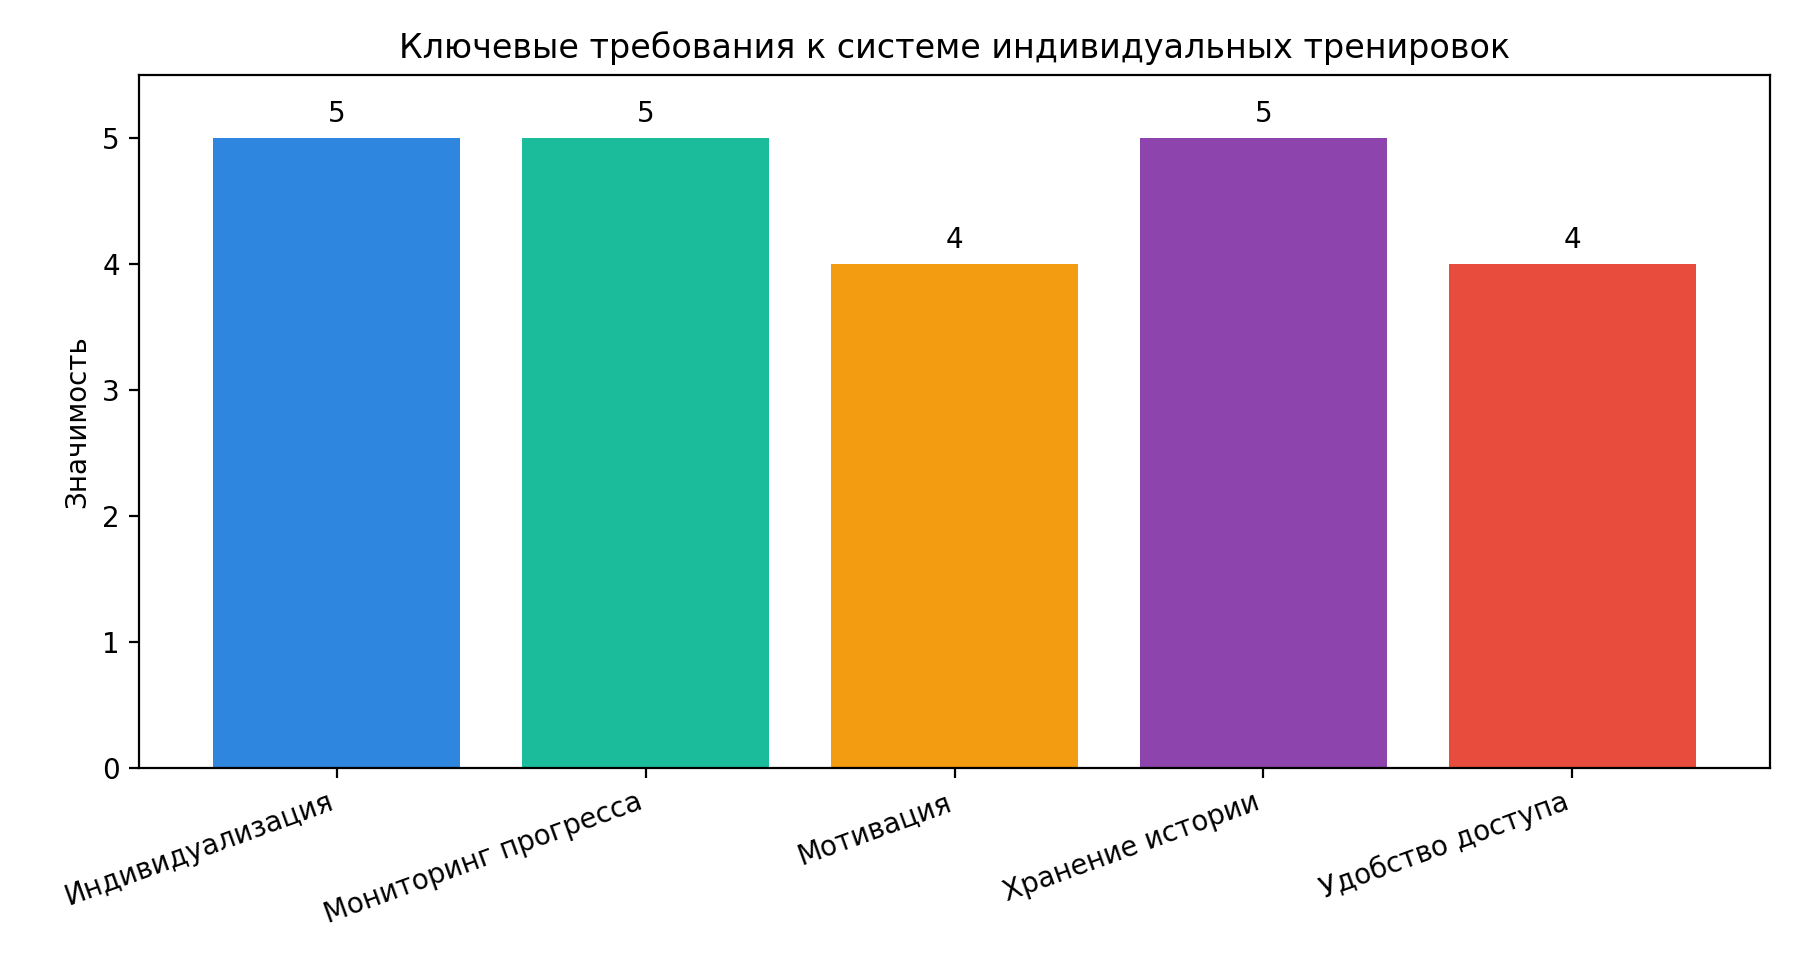
\includegraphics[width=0.9\linewidth]{fitness_analysis_factors.png}
	\caption{Ключевые требования к системе индивидуальных тренировок (оценка значимости)}
	\label{fig:fitness-factors}
\end{figure}

Из рисунка ~\ref{fig:fitness-factors} видно, что приоритет следует отдавать функциям, связанным с индивидуальным планированием и анализом прогресса. Именно эти возможности формируют практическую ценность системы для пользователя и отличают ее от простого справочника упражнений.

\subsection{Классификация цифровых решений в области физической активности}

Современные цифровые решения для фитнеса и контроля физической активности можно разделить на несколько основных групп.

\subsubsection{Тренировочные дневники и трекеры активности}

Данные приложения ориентированы на учет упражнений, подходов, повторений, веса отягощений, времени выполнения и частоты тренировок. Их сильная сторона заключается в удобном журналировании и последующем анализе динамики. Однако такие системы часто ограничиваются фиксацией результата и не всегда предлагают гибкую модель построения индивидуального плана.

\subsubsection{Сервисы контроля питания}

Приложения для учета питания позволяют отслеживать калорийность, белки, жиры и углеводы, а также сравнивать фактическое потребление с целевыми значениями. Они полезны при работе с задачами снижения или набора массы, но обычно слабо связаны с тренировочной частью и не формируют единую картину физической подготовки пользователя.

\subsubsection{Экосистемы носимых устройств}

Фитнес-браслеты, умные часы и связанные с ними мобильные приложения предоставляют данные о пульсе, шаговой активности, сне и иногда о тренировочной нагрузке. Такие решения удобны за счет автоматического сбора информации, однако их функциональность зависит от конкретного оборудования, а логика работы часто привязана к закрытой экосистеме производителя.

\subsubsection{Социальные и мотивационные платформы}

Некоторые цифровые продукты делают акцент на челленджах, рейтингах, сообществах и публичной демонстрации результатов. Это повышает вовлеченность, но может быть недостаточно полезно для точного планирования тренировочного процесса. Кроме того, чрезмерная ориентация на социальное сравнение не всегда способствует устойчивому результату.

Таким образом, на практике существует разрыв между приложениями для учета активности, дневниками питания и мотивационными платформами. Это обосновывает разработку системы, объединяющей несколько функций в едином интерфейсе.

\subsection{Сравнение архитектурных решений}

При проектировании информационной системы для составления индивидуального плана тренировок возможны различные архитектурные подходы.

Подход только клиент подходит для простых локальных решений, но не обеспечивает надежное хранение данных, совместную работу с несколькими устройствами и централизованное управление учетными записями. Такой вариант удобен для прототипов, но ограничен при дальнейшем развитии системы.

Подход клиент + сервер + база данных является наиболее рациональным для рассматриваемой задачи. Он позволяет разделить пользовательский интерфейс, бизнес-логику и хранение данных, обеспечить авторизацию, синхронизацию прогресса и расширяемость системы. Именно такой вариант соответствует целям преддипломной практики и дает возможность реализовать полноценный учебный программный продукт.

Микросервисная архитектура, хотя и является современной и масштабируемой, для учебного проекта избыточна. Она увеличивает сложность развертывания, сопровождения и тестирования, не давая существенных преимуществ на данном этапе разработки.

Наиболее рациональным вариантом является клиент-серверная архитектура с базой данных. Она обеспечивает разделение интерфейса, бизнес-логики и хранения информации, а также позволяет реализовать авторизацию, синхронизацию пользовательских данных и дальнейшее расширение функциональности.

\subsection{Пользовательские сценарии и функциональные потребности}

Основной пользователь системы -- человек, который хочет самостоятельно заниматься физической активностью и контролировать результат. Для такого пользователя наиболее типичны следующие сценарии:
\begin{itemize}
	\item регистрация и авторизация в системе;
	\item создание и редактирование профиля с индивидуальными параметрами;
	\item получение персонального плана тренировок;
	\item ведение дневника выполненных упражнений;
	\item просмотр истории, статистики и динамики результатов;
	\item использование дополнительных разделов, связанных с питанием, поддержкой и социальным взаимодействием.
\end{itemize}

Из этих сценариев следует, что система должна обеспечивать не только ввод и хранение данных, но и удобную навигацию, быстрый доступ к ключевым функциям и возможность последующего расширения без полной переработки архитектуры.

\subsection{Требования к качеству данных и безопасности}

Так как система работает с персональными данными пользователя, к ней предъявляются требования по защите информации. Минимально необходимыми являются разграничение доступа к учетной записи, безопасное хранение паролей в виде хэшей, защита пользовательских данных от несанкционированного просмотра и корректная работа механизма аутентификации.

С точки зрения качества данных важно обеспечить целостность и актуальность информации. Данные о тренировках и результатах должны сохраняться в структурированном виде, чтобы их можно было использовать для построения истории прогресса и дальнейшего анализа. Для этого целесообразно применять реляционную модель данных и хранить основные сущности в отдельных таблицах.

С точки зрения интерфейса система должна быть понятной, предсказуемой и не перегруженной лишними действиями. Для пользователя, который занимается спортом регулярно, особенно важны быстрое внесение данных, наглядность результата и отсутствие избыточной сложности.

\subsection{Обзор аналогов}

На рынке существует множество цифровых решений, связанных с фитнесом и питанием, однако большинство из них решает только одну часть задачи. Одни приложения ориентированы на учет тренировок, другие -- на дневник питания, третьи -- на социальную мотивацию или работу с носимыми устройствами. При этом редко встречается решение, в котором в одном продукте объединены индивидуальный план тренировок, мониторинг результата, вспомогательные мотивационные механизмы и удобное веб-управление. Сравнительная характеристика функций аналогов представлена в таблице ~\ref{tab:analog-comparison}.

\begin{xltabular}{\textwidth}{|p{3.2cm}|X|X|}
	\caption{Сопоставление коммерческих решений и разрабатываемой информационной системы\label{tab:analog-comparison}}\\ \hline
	\centrow Решение & \centrow Основной функционал & \centrow Замечание для сопоставления с целевой ИС \\ \hline
	\endfirsthead
	\continuecaption{Продолжение таблицы \ref{tab:analog-comparison}}
	\centrow Решение & \centrow Основной функционал & \centrow Замечание для сопоставления с целевой ИС \\ \hline
	\finishhead
	
	Strong & План и учёт силовых тренировок, история подходов, базовая аналитика & Нет учёта питания, социального раздела и работы через браузер; расширенные возможности частично за подписку \\ \hline
	Hevy & Аналогичный учёт тренировок с акцентом на программы и статистику & Питание и полноценный социальный модуль не являются ядром продукта; веб-клиент ограничен; freemium-модель \\ \hline
	MyFitnessPal & Дневник питания, калории и нутриенты, штрихкоды, интеграции & План силовых тренировок и связанная аналитика прогресса не являются центральной задачей продукта \\ \hline
	Strava & Кардионагрузки, GPS-треки, сегменты, соревновательная мотивация & Фокус на беге и велосипеде; силовой зал и рацион как единый контур не объединены \\ \hline
	JEFIT & Программы упражнений, учёт тренировок, есть веб-доступ & Питание и сеть как у целевой ИС представлены слабо; часть функций за подпиской \\ \hline
	Lose It! & Контроль питания, цели по калориям, поддержка привычек & Как и у других дневников питания, тренировочный контур неразвит \\ \hline
	Наша ПИС & План и дневник тренировок, учёт прогресса, раздел питания, социальные механизмы, веб-клиент в одной системе & Учебная ИС; развитие ограничено учебной постановкой, а не лакунами по видам функций \\ \hline
\end{xltabular}

Наиболее близкие по функциональности системы, как правило, либо слишком узкоспециализированы, либо требуют подписки, либо завязаны на конкретную платформу. Поэтому разработка учебной информационной системы является обоснованной: она позволяет реализовать ключевые функции в одном программном комплексе и продемонстрировать полный цикл проектирования.

\subsection{Актуальность разработки}

Актуальность разработки обусловлена ростом интереса к цифровым сервисам для здоровья и физической активности, а также потребностью пользователей в простых и понятных инструментах самостоятельного контроля тренировочного процесса. Современный пользователь ожидает, что система не только сохранит данные, но и поможет организовать занятия, увидеть прогресс и поддерживать мотивацию на протяжении длительного времени.

Для преддипломной практики разработка подобной системы представляет интерес с точки зрения программной инженерии, так как включает проектирование предметной области, выбор архитектуры, разработку пользовательского интерфейса, организацию хранения данных и реализацию механизмов авторизации и обработки пользовательской информации.


\section{Техническое задание}

\subsection{Основание для разработки}

Основанием для разработки является задание на выпускную квалификационную работу бакалавра <<Приложение для составления тренировочного плана и отслеживания прогресса>>.

\subsection{Цель и назначение разработки}

Основной задачей выпускной квалификационной работы является разработка и тестирование программно-информационной системы для индивидуального планирования тренировок и отслеживания прогресса.

Целью разработки является создание работоспособного многопользовательского веб-приложения, позволяющего составлять и выполнять персональные планы тренировок, фиксировать результаты и распределение нагрузки по группам мышц, вести дневник питания с учётом калорийности и КБЖУ, а также поддерживать мотивацию за счёт модуля психологической поддержки, аватара с системой опыта и элементов социального взаимодействия.

Задачами данной разработки являются:
\begin{itemize}
	\item изучение предметной области и сопоставление архитектурных подходов для веб-приложений с учётом требований к хранению персональных данных и синхронизации между устройствами;
	\item проектирование программной системы;
	\item проектирование интерфейса пользователя;
	\item реализация аутентификации и управления профилем;
	\item реализация модуля тренировок;
	\item реализация модуля питания, модуля поддержки и модуля цифрового аватара;
	\item реализация социальной ленты (посты, комментарии, лайки, реакции) и клиентского модуля взаимодействия с ней;
	\item тестирование ключевых сценариев (регистрация и вход, сохранение плана и тренировки, дневник питания, публикации в ленте) и отладка взаимодействия клиента с API.
\end{itemize}

\subsection{Функциональные требования}

Ниже приведен перечень функций, которые должно обеспечивать приложение.

Аутентификация и профиль. Данный блок включает следующие возможности:
\begin{itemize}
	\item регистрация пользователя и вход в систему;
	\item управление параметрами профиля (личные данные, цели, контакты при необходимости, загрузка фотографии).
\end{itemize}

Тренировки. Приложение должно предоставлять пользователю следующие функции для работы с тренировками:
\begin{itemize}
	\item составление, редактирование и сохранение индивидуальных планов тренировок с разбиением по дням цикла;
	\item доступ к каталогу упражнений с группировкой по группам мышц и разделением силового и кардио-компонентов при планировании;
	\item использование готовых шаблонных программ;
	\item выполнение тренировки по выбранному плану и дню и фактическая фиксация результатов;
	\item ведение истории выполненных тренировок;
	\item визуальный анализ прогресса (графики, календарь, распределение нагрузки, рекомендации по нагрузке в общем виде).
\end{itemize}

Питание и КБЖУ. Для отслеживания питания предусмотрены следующие возможности:
\begin{itemize}
	\item ведение дневника приёмов пищи с привязкой к календарной дате;
	\item ручной ввод продуктов и блюд, в том числе пользовательских;
	\item расчёт и отображение калорийности и КБЖУ за день, сводок и диаграмм динамики;
	\item доступ к справочнику продуктов с поиском и выбором позиций.
\end{itemize}

Модули поддержки, аватар и дополнительная мотивация. В приложении также реализованы:
\begin{itemize}
	\item раздел поддержки пользователя с вспомогательными материалами и чекинами;
	\item модуль «Аватар» (цифровой персонаж, уровень и отображение активности).
\end{itemize}

Социальное взаимодействие. Для общения и обмена опытом между пользователями предназначены:
\begin{itemize}
	\item общая лента сообщений пользователей установки приложения с публикациями, комментариями и реакциями;
	\item поиск и упорядочивание сообщений для удобства просмотра;
	\item использование профильных данных (в т.ч. изображений) для отображения участников при обмене сообщениями.
\end{itemize}

\subsection{Роли пользователей}

До успешной аутентификации пользователь работает с экраном входа и регистрации. После входа открывается основной интерфейс с сохранением данных на сервере. Условно выделяются две роли.

Неавторизованный пользователь. Видит экран входа и регистрации.

Зарегистрированный пользователь. После входа получает полный доступ к функциям клиента: планы и журнал тренировок, питание, профиль, поддержка, аватар, социальная лента, сохранение и синхронизация данных учётной записи между сеансами работы.

Роль назначается автоматически после успешной регистрации или входа.

\subsection{Требования к интерфейсу}

Интерфейс реализуется как одностраничное приложение в браузере: до аутентификации доступен только экран входа и регистрации; после входа отображается единый каркас с постоянной верхней панелью и областью контента выбранного раздела. Переключение модулей выполняется без перезагрузки документа (кроме принудительной перезагрузки после регистрации в реализации клиента). Для иллюстрации структуры в документе используются два макета: экран авторизации и развёртка главного окна на примере модуля <<Тренировки>> (рисунки~\ref{fig:tzuiauthorization} и~\ref{fig:tzuitraining}).

\subsubsection{Экран авторизации и регистрации}

До входа пользователь видит карточку с заголовком и кратким пояснением назначения входа. Предусмотрено переключение двух режимов вкладками: <<Вход>> и <<Регистрация>>; активная вкладка визуально выделена. В режиме <<Вход>> (рисунок~\ref{fig:tzuiauthorization}) показываются поля <<Логин>> и <<Пароль>> и кнопка подтверждения (<<Войти>>). В режиме <<Регистрация>> дополнительно отображаются фамилия, имя, дата рождения (маска ДД.ММ.ГГГГ), выбор пола двумя кнопками. Сообщения об ошибках валидации и ответа сервера выводятся в той же карточке. Оформление согласовано с цветовой темой приложения.

\begin{figure}[H]
	\centering
	
\includegraphics[width=0.82\linewidth]{tz_ui_authorization.png}
	\caption{Макет экрана авторизации (режим <<Вход>>)}
	\label{fig:tzuiauthorization}
\end{figure}

\subsubsection{Главное окно: верхняя панель и пример раздела <<Тренировки>>}

После входа в верхней части экрана отображается навигационная панель (на макете рисунок~\ref{fig:tzuitraining}): переключатели пяти разделов -- <<Тренировки>>, <<Питание>>, <<Социальные сети>>, <<Поддержка>>, <<Аватар>> -- и блок учётной записи (логин, значок пользователя, вызов профиля, смена светлой\,/\,тёмной темы, выход). Активный раздел подчёркивается относительно остальных. На приведённом макете выбран раздел <<Тренировки>>; та же панель используется для перехода к остальным модулям, заменяя только содержимое рабочей области.

В колонках под панелью раскрывается функциональность <<Тренировки>>. Слева -- <<Мои планы>>, каталог упражнений по группам мышц, шаблоны программ, сводка по текущему плану и числу упражнений; внизу допускаются подсказки о серверном сохранении, теме оформления и графиках прогресса. В центре -- выбранный день плана со списком упражнений (название, группа мышц), поиск по упражнениям дня, добавление упражнения, запуск выполнения тренировки, привязка типа нагрузки, переход к графику по упражнению, удаление позиции. Справа -- аналитика: переключение <<Прогресс>>\,/\,<<Календарь>>, график нагрузки по группам мышц, блок рекомендаций по прогрессии. Компоновка поддерживает цепочку планирование -- выполнение -- анализ; при ограничении высоты окна допускается вертикальная прокрутка блоков.

\begin{figure}[H]
	\centering
	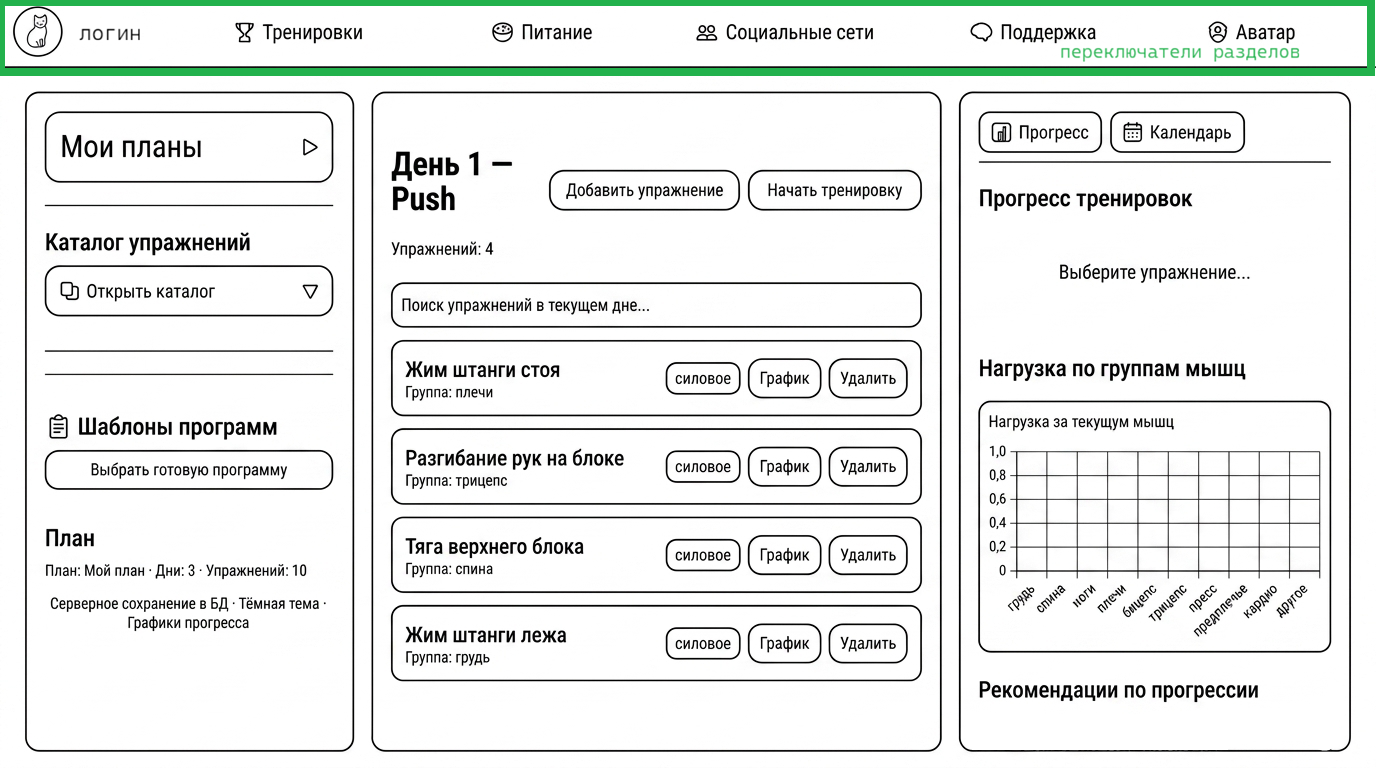
\includegraphics[width=0.95\linewidth]{tz_ui_training.png}
	\caption{Макет главного окна: панель разделов и интерфейс модуля <<Тренировки>>}
	\label{fig:tzuitraining}
\end{figure}

\subsubsection{Разделы <<Питание>>, <<Социальные сети>>, <<Поддержка>>, <<Аватар>> и профиль}

Пункты <<Питание>>, <<Социальные сети>>, <<Поддержка>> и <<Аватар>> открываются с верхней панели (см. переключатели на рисунке~\ref{fig:tzuitraining}); иллюстрация содержимого этих модулей в настоящем разделе не приводится -- в рабочей области отображаются специализированные экраны. В <<Питание>> -- дневник приёмов на дату, приёмы со сворачиванием, поиск и выбор продуктов, показатели калорийности и КБЖУ, при необходимости график по дням. В <<Социальные сети>> -- лента постов, ввод публикаций и комментариев, элементы реакций. В <<Поддержка>> -- советы, чекины, опциональный календарь состояний и вспомогательные материалы. В <<Аватар>> -- цифровой персонаж, уровень и метрики активности. Профиль пользователя и загрузка фотографии доступны из элементов учётной записи на панели; в профиле задаются дополнительные личные данные.

\subsection{Сценарии использования}

Для наглядного представления типовых действий пользователей по ролям на рисунке~\ref{fig:diagramm} приведены диаграммы вариантов использования для неавторизованного и авторизованного пользователей соответственно.

\begin{figure}[H]
	\centering
	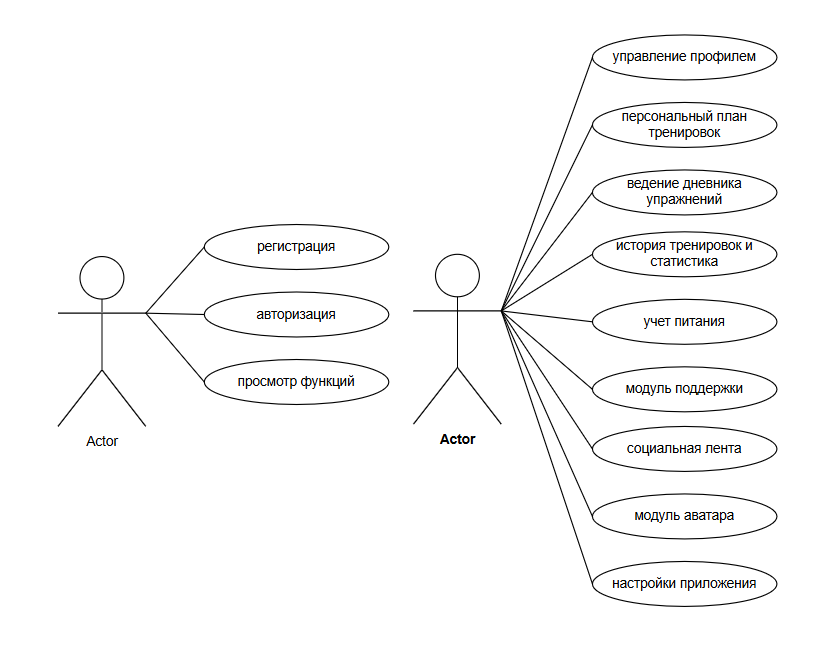
\includegraphics[width=0.90\linewidth]{images/diagramm.png}
	\caption{Диаграммы вариантов использования}
	\label{fig:diagramm}
\end{figure}

\subsubsection{Регистрация нового пользователя}

Пользователь открывает приложение и попадает на экран входа. Для создания новой учётной записи переключается на вкладку <<Регистрация>>, после чего на экране появляется расширенный набор полей: помимо имени входа и пароля система предлагает указать фамилию, имя, дату рождения и пол. Заполнив необходимые поля, человек отправляет регистрационную анкету.

Система проверяет, что информация представлена в допустимом виде: что обязательные поля не пустые, что дата рождения выглядит корректно, что логин и пароль удовлетворяют простым ограничениям по минимальной длине или формату, принятым в приложении. Если уже существует пользователь с таким же именем входа, об этом сообщают понятным текстом, чтобы человек мог выбрать другое имя входа или войти под существующей учётной записью.

При успешной регистрации пользователь становится авторизованным: открывается основное окно приложения с разделами тренировок, питания, социальной активности и прочего функционала. Часть сведений, не обязательных при первоначальной анкете, человек имеет возможность добавить позже в профиле, когда будет удобно.

\subsubsection{Вход в систему}

Пользователь, ранее прошедший регистрацию, выбирает вкладку <<Вход>>, вводит своё имя входа и пароль и подтверждает действие.

Если имя входа и пароль соответствуют ранее зарегистрированной учётной записи этого пользователя, система показывает главный интерфейс с сохранёнными его данными.

Если вход не удался -- например из-за неверного пароля -- приложение сообщает об этом без раскрытия лишних деталей, чтобы исключить злоупотребления со стороны посторонних, и пользователь может повторить ввод или воспользоваться регистрацией, если учётную запись ещё не создавал.

\subsubsection{Заполнение и изменение профиля}

Из основного интерфейса пользователь переходит к разделу личной учётной записи и открывает экран профиля. Здесь он может уточнить или изменить параметры тела и целей, добавить текстовые пояснения о фитнес-задаче и уровне активности, при необходимости указать город, контактные данные или краткие медицинские заметки, которые сам считает уместными хранить в приложении для собственной ориентации. Допускается загрузка фотографии для отображения в интерфейсе.

После сохранения изменений система показывает обновлённые данные там, где профиль представлен пользователю и там, где визуально обозначаются участники в других частях приложения -- например в социальной ленте. Если какие-либо значения указаны недопустимо или сохранить их не удалось, пользователь получает понятное сообщение и может поправить анкету.

\subsubsection{Создание и корректировка индивидуального плана тренировок}

Пользователь переходит в раздел <<Тренировки>> и находит блок со своими сохранёнными планами. Он может начать новый цикл занятий <<с чистого листа>>, задав собственное имя плана и число тренировочных дней в недельном\,/\,циклическом режиме, либо взять готовый шаблон программы как отправную точку и затем отредактировать её под себя.

Далее из каталога упражнений, сгруппированного по области тела\,/\,мышечным группам и типу нагрузки, пользователь переносит нужные упражнения на выбранные дни. Для каждой позиции задаёт запланированное число подходов, повторений и\,/\,или рабочий вес, при необходимости переименовывает или дублирует целый день\,/\,фрагмент плана для ускорения настройки. Готовое расписание сохраняется под выбранным именем.

Система отображает план в общем списке, позволяет переключаться между сохранёнными вариантами, открыть конкретный день перед тренировкой и при необходимости вернуться к редактированию: добавить упражнение, удалить позицию, изменить параметры без потери уже накопленной истории по другим занятиям.

\subsubsection{Выполнение тренировки по плану}

Перед началом занятий пользователь указывает, каким планом он пользуется и какой это день в цикле. На экране появляется список запланированных упражнений с ориентирами по подходам.

В ходе тренировки человек выполняет подходы и фиксирует факт: реальное число повторений, массу отягощения или иные показатели, которые поддерживаются интерфейсом для данного типа упражнения. Система по возможности подсказывает значения из прошлых успешных тренировок, чтобы не вводить одно и то же заново.

По окончании серии упражнений пользователь явно завершает занятие. Тогда приложение считает день выполненным, заносит сведения в журнал тренировок и обновляет все экраны, где отображается прогресс: графики, календарь, суммарные показатели. Дополнительно накопление регулярных занятий может отображаться через модуль мотивации с цифровым аватаром.

\subsubsection{Ведение дневника питания}

В разделе <<Питание>> пользователь указывает интересующий календарный день -- например текущее число -- чтобы вести дневник строго <<за сегодня>> или просмотреть\,/\,дополнить прошлые даты.

Внутри суток добавляются отдельные приёмы пищи: завтрак, обед, перекуски -- названия и число блоков зависят от привычек пользователя. В каждый блок помещаются позиции: либо выбранный из приложенного справочника продукт или блюдо, либо собственное описание с приблизительной порцией, если нужной записи ещё нет.

Приложение суммирует калорийность и долю белков, жиров и углеводов по дню, показывает итог в компактном виде и может нарисовать тенденцию за несколько дней подряд, чтобы человек видел общую картину, а не только одну строку счёта. Приём пищи можно сворачивать после заполнения, чтобы не засорять экран во время активного расчёта рациона.

\subsubsection{Раздел поддержки и отметки самочувствия}

Открывая раздел <<Поддержка>>, пользователь получает доступ к текстовым советам, подсказкам по восстановлению и регулярности тренировок, а также к простым действиям вроде чекина за день: отметить настроение, отметить факт тренировки или отдыха. Это необязательный сценарий, но если человек его использует, система сохраняет записи как личную хронику и может показывать их только ему же при последующих визитах.

\subsubsection{Модуль <<Аватар>> и наблюдение за <<опытом>>}

Пользователь переключается на раздел <<Аватар>>, где видит оформленного персонажа -- иллюстративную <<награду>> за регулярность и объём нагрузок. По мере сохранённых и завершённых тренировок уровень или стадия персонажа обновляется; приложение сообщает это ненавязчиво через визуальные изменения и краткие подписи, без превращения модуля в отдельную игру. Человек может заглянуть туда перед или после недели занятий, чтобы зафиксировать ощущение прогресса.

\subsubsection{Активность в социальной ленте}

В разделе <<Социальные сети>> перед пользователем открыта общая для данной установки приложения лента публикаций. Он может прочитать записи других зарегистрированных участников с их именами входа\,/\,никами\,/\,маленькими изображениями профилей, переходить к комментированию тем, которые его заинтересовали.

Собственную мысль о тренировке, результате\,/\,переживании пользователь может оформить как новый пост после ввода текста в предназначенной для этого области. Если лента длинная, для удобства предусмотрены поиск по словам и упорядочивание сообщений -- например сначала самые новые или наоборот старые, в зависимости от режима интерфейса.

Оценивая содержание, человек ставит символический <<лайк>>, выбирает эмодзи-реакцию среди набора приложения или оставляет ответ в виде цепочки комментариев под постом. Если какие-то авторы кажутся полезнее остальных, пользователь может отметить их внутри приложения как приоритетных для быстрой фильтрации при следующих визитах. Автор имеет возможность временно закрепить свой пост над лентой, если такая возможность поддерживается в интерфейсе.

Система отражает результат действий человека сразу в ленте: новый пост, обновившийся список реакций, новый порядок при смене сортировки. Запрещённые или недопустимые по правилам приложения сообщения приложение не должно добавлять; при технических сбоях пользователь получает предупреждение о неудаче операции без потери уже введённого текста, где это возможно.

\subsubsection{Просмотр статистики и истории результатов}

Пользователь возвращается в раздел <<Тренировки>> или использует уже знакомые панели анализа и там выбирает интересующий показатель: конкретное упражнение для просмотра динамики силового результата, сводную диаграмму распределения нагрузки по группам мышц, календарь с отмеченными завершёнными днями. Это позволяет ответить на вопросы <<что уже работает>>, <<равномерно ли распределены нагрузки>>, <<как часто в последнее время выполняются планы>>.

При необходимости для мотивации человек дополнительно открывает <<Аватар>> и видит связку между наблюдаемым прогрессом в числах и наглядной <<выдачей>> персонажа. Отдельным запросом к питательному журналу тот же человек может сопоставить графики тренировочной активности и динамику калорийности за неделю, если оба режима заполняются регулярно -- приложение просто параллельно хранит и показывает эти два контура данных.

\subsection{Требования к оформлению документации}

Разработка программной документации и программного изделия должна производиться согласно ГОСТ~19.102-77 и ГОСТ~34.601-90. Единая система программной документации.

\section{Технический проект}

\subsection{Общая характеристика организации решения задачи}

Система построена по схеме <<клиент -- сервер>>. Сервер на Node.js принимает HTTP-запросы: проверяет логин и пароль, выдаёт и проверяет JWT, выполняет запросы к PostgreSQL, собирает ответы социальной ленты в JSON и отдаёт их клиенту. Статические файлы интерфейса (HTML, CSS, JavaScript, ресурсы) отдаются из каталога фронтенда тем же процессом. Если приходит GET по пути, для которого нет отдельного обработчика, сервер отдаёт главную HTML-страницу клиента; маршрутизация внутри приложения дальше выполняется на стороне браузера (одностраничное приложение).

Условно выделяются три уровня:
\begin{enumerate}
	\item Клиент: работа с DOM, сценарии с суффиксом <<.module.js>>, локальное хранилище браузера, построение графиков с помощью Chart.js.
	\item Сервер приложения: маршруты Express, проверка входных данных, ограничение числа запросов на регистрацию и вход.
	\item Данные: таблицы PostgreSQL, доступ через пул соединений библиотеки pg.
\end{enumerate}

После успешного входа клиент в последующих запросах к защищённым URL передаёт JWT в заголовке Authorization. Обработчик маршрута извлекает из токена userId и username и подставляет их в объект запроса. Дополнительные данные пользователя (например, настройки экранов, сохранённые на клиенте) синхронизируются с таблицей user\_storage.

На рисунке~\ref{fig:componentinteraction} показана общая схема взаимодействия компонентов развёрнутой системы: авторизованный пользователь работает через браузер с одностраничным приложением; запросы к REST API и раздача статики выполняются сервером Node.js\,/\,Express; персистентные данные учётных записей, профиля, пользовательского хранилища и социальной ленты хранятся в PostgreSQL; справочные JSON-файлы и библиотека Chart.js подгружаются из статического каталога фронтенда (тот же HTTP-сервер).

\begin{figure}[H]
	\centering
	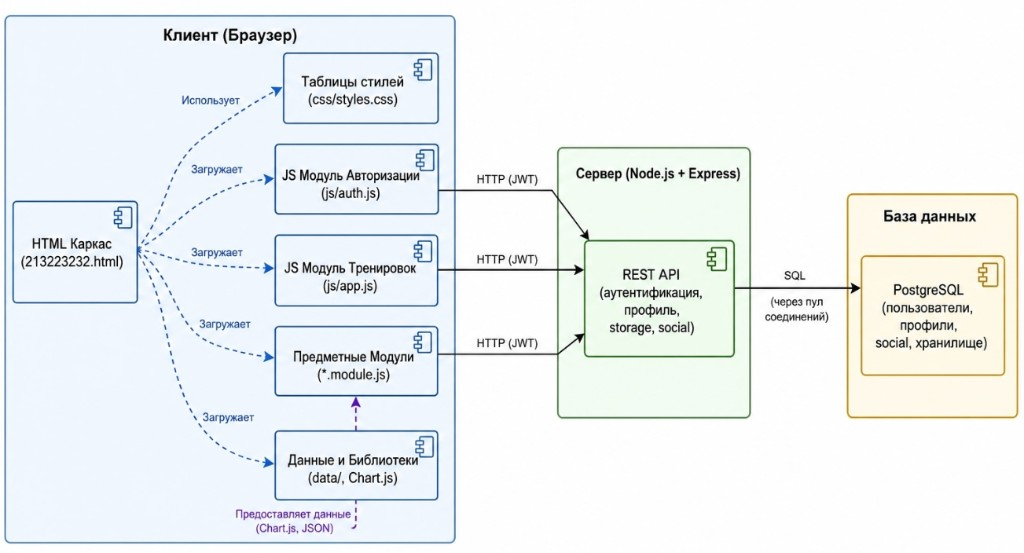
\includegraphics[width=0.98\textwidth]{images/component_interaction}
	\caption{Диаграмма компонентов программно-информационной системы Fitness Life}
	\label{fig:componentinteraction}
\end{figure}

\subsection{Обоснование выбора технологии проектирования}

Стек выбирался из требований задания: нужны реляционная БД с явной схемой, REST API, сервер на JavaScript и возможность отдать готовый статический фронтенд без обязательной сборки через отдельный бандлер.

\subsection{Структура клиентской части}

В клиентской части проекта выделяются следующие основные файлы:
\begin{itemize}
	\item \texttt{213223232.html} -- основная HTML-страница;
	\item \texttt{css/styles.css} -- таблица стилей приложения;
	\item \texttt{js/auth.js} -- клиентский слой авторизации и подготовки состояния;
	\item \texttt{js/app.js} -- основной модуль тренировочного интерфейса;
	\item \texttt{modules/profile.module.js} -- модуль профиля;
	\item \texttt{modules/nutrition.module.js} -- модуль питания;
	\item \texttt{modules/psychology.module.js} -- модуль психологической поддержки;
	\item \texttt{modules/social.module.js} -- модуль социальной ленты;
	\item \texttt{modules/avatar.module.js} -- модуль аватара;
	\item \texttt{data/mental-advice.json} -- данные для раздела поддержки;
	\item \texttt{js/vendor/chart.umd.min.js} -- локальная версия Chart.js.
\end{itemize}

Файловая декомпозиция клиента соответствует принципу единственной ответственности: авторизация отделена от тренировочной логики, а предметные разделы (профиль, лента, питание и др.) вынесены в подключаемые модули. Такой подход облегчает сопровождение -- правки в социальной ленте не должны затрагивать алгоритмы построения графиков -- и отражает зрелую практику организации кода в браузере даже при отказе от тяжёлых SPA-фреймворков в пользу <<склеивания>> логики вручную.

Модуль \texttt{avatar.module.js} на клиенте пересчитывает опыт и уровень персонажа, опираясь на данные тренировок (\texttt{app.js}, история подходов), дневника питания (\texttt{nutrition}) и чекинов раздела <<Поддержка>> (\texttt{psychology}); социальная лента в этот расчёт не входит.

\subsection{Организация HTML-страницы}

Основная HTML-страница содержит два ключевых корневых блока: \texttt{authRoot} и \texttt{appRoot}. Первый используется для отображения формы авторизации и регистрации. Второй содержит основной интерфейс и по умолчанию скрывается до завершения входа пользователя.

Внутри \texttt{appRoot} находится верхняя панель: кнопка профиля (открывает отдельную вкладку \texttt{profile-tab}), виртуальный аватар пользователя (\texttt{virtualAvatarMount}), имя пользователя и ряд вкладок \texttt{data-tab}.

Тренировочная вкладка содержит трёхколоночную разметку. Остальные предметные разделы имеют контейнеры \texttt{\#nutrition-tab}, \texttt{\#social-tab}, \texttt{\#psychology-tab}, \texttt{\#avatar-tab}, куда через \texttt{AppModules.*.render()} монтируются модули. Внизу корня приложения описаны элементы общих модальных окон (\texttt{\#modal}, \texttt{\#confirmModal}, \texttt{\#alertModal}) для единого визуального поведения.

\subsection{Вкладочный интерфейс}

Вкладочный интерфейс позволяет разместить большое количество функций в одном приложении. Каждая вкладка соответствует отдельной предметной области:
\begin{itemize}
	\item тренировки -- основная работа с планами и упражнениями;
	\item питание -- дневник рациона, калории и календарный обзор приёмов пищи;
	\item социальные сети -- сообщество пользователей, поиск по ленте, сортировка и реакции;
	\item поддержка -- ментальный ассистент, чекин, советы из JSON и справочник контактов помощи;
	\item аватар -- цифровой персонаж с уровнями начисления опыта;
	\item профиль (без собственной кнопки в таб-ряду) -- форма данных пользователя из панели инструментов.
\end{itemize}

При переключении вкладок JavaScript изменяет CSS-классы активных элементов. Это позволяет не перезагружать страницу и мгновенно менять отображаемый раздел.

\subsection{Основной модуль тренировок}

Основной тренировочный модуль реализован в файле \texttt{app.js}. В нём определён каталог упражнений по группам мышц:
\begin{itemize}
	\item грудь;
	\item спина;
	\item ноги;
	\item плечи;
	\item бицепс;
	\item трицепс;
	\item пресс;
	\item предплечье;
	\item кардио;
	\item другое.
\end{itemize}

Каталог используется для быстрого выбора упражнения при составлении плана. Такое решение удобно для пользователя, потому что ему не нужно каждый раз вводить название упражнения вручную.

Основные функции тренировочного модуля:
\begin{itemize}
	\item создание, выбор, сохранение и удаление плана (с подтверждением деструктивных операций);
	\item генерация списка тренировочных дней по заданному количеству;
	\item сворачивание блока <<Мои планы>> (состояние свёртки может сохраняться в \texttt{localStorage});
	\item интерактивный каталог \texttt{EXERCISES\_BY\_MUSCLE} с раскрытием групп и выбором упражнений;
	\item набор стандартных программ в объекте \texttt{TRAINING\_TEMPLATES} (верх/низ split, push/pull/legs, full body, жиросжигание, $5\times5$, домашняя минимальная и др.), применение выбранной программы перезаписывает текущие дни плана и уведомляет пользователя через \texttt{alertModal};
	\item поле поиска \texttt{\#searchEx} для фильтрации упражнений только в активном дне;
	\item добавление упражнения через модальное окно (тип нагрузки, мышечная группа, шаблон подходов);
	\item режим <<Начать тренировку>> с фиксацией даты, набора подходов и сохранением истории (\texttt{trainingWorkouts\_v4});
	\item подвкладка <<Прогресс>>: графики Chart.js по выбранному упражнению, столбчатая диаграмма нагрузки по группам мышц, эвристические рекомендации прогрессии;
	\item подвкладка <<Календарь>>: отрисовка сетки месяца, выбор дня, отображение всех сохранённых тренировок дня и кнопка полной очистки истории (с подтверждением).
\end{itemize}

Модуль использует ключи \texttt{trainingPlans\_v3}, \texttt{trainingWorkouts\_v4}, \texttt{trainingLastSetByExercise\_v1} для раздельного хранения структуры планов, истории выполнения и последних введённых значениях повторов/веса.

\subsubsection{Глобальные модальные окна}

Общая инфраструктура диалогов реализована в HTML-тенях страницы. Функции \texttt{openModal}/\texttt{closeModal} заполняют \texttt{\#modalContent} и включают класс \texttt{active} для всей шторки; \texttt{confirmModal} задаёт текст вопроса и колбэки <<Да>>/<<Отмена>>; \texttt{alertModal} выводит короткое сообщение об ошибке или успешном действии (например, применение шаблона программы). Такой подход унифицирует обратную связь и снижает дублирование вёрстки.

\subsection{Графики прогресса}

Для визуализации прогресса используется библиотека Chart.js. Графики позволяют пользователю воспринимать данные быстрее, чем при просмотре таблиц или длинных списков. Например, по графику проще увидеть изменение веса, количества повторений или объёма тренировок.

Помимо линейных графиков по упражнению, в правой панели строится агрегированная диаграмма нагрузки по группам мышц (на основе выполненных тренировок) и выводится текстовый блок рекомендаций по прогрессии нагрузок.

В клиентском коде предусмотрена локальная версия библиотеки. Если она недоступна, может быть использована резервная загрузка с CDN. Такой подход повышает устойчивость клиентской части.

\subsection{Модуль авторизации}

Модуль \texttt{auth.js} отвечает за отображение авторизационного слоя, хранение клиентского признака входа и подготовку данных перед запуском основного интерфейса. Важной особенностью является блокировка запуска основного приложения (\texttt{window.\_\_APP\_LOCKED\_\_}) до окончания подготовки состояния, чтобы пользователь не видел <<полупустую>> разметку и дублирующие формы. При входе выполняется гидратация пользовательского \texttt{localStorage} с сервера (в отчёте без детализации серверной реализации), чтобы данные планов и дневников не <<перетекали>> между учётными записями на одном устройстве.

Внутри модуля используются ключи \texttt{appAuthToken\_v1} и \texttt{appAuthUser\_v1}. Они позволяют сохранить информацию о текущем пользователе на стороне браузера.

\subsection{Модуль профиля}

Модуль профиля отвечает за отображение и редактирование пользовательских данных. Он связан с верхней панелью: при изменении фотографии профиля должны обновляться аватар, панель профиля и элементы социальной ленты.

Клиентская часть профиля должна выполнять:
\begin{itemize}
	\item отображение заполненных полей и переключение в режим редактирования;
	\item обработку изменения полей с разбором даты рождения в формате дд.\,мм.\,гггг;
	\item проверку корректности значений на уровне формы;
	\item передачу изображения аватара другим модулям;
	\item генерацию события обновления фотографии;
	\item переключение цветовой темы оформления и выход из аккаунта (клиентская очистка токена и состояния).
\end{itemize}

\subsection{Модуль питания}

Модуль \texttt{nutrition.module.js} реализует полноэкранный дневник питания: календарь выбора дня, список приёмов пищи с добавлением позиций из справочника или вручную, модальные формы для нового приёма и для пользовательского продукта (БЖУ и ккал на 100\,г), учёт сворачивания карточек приёмов. Боковая панель отображает кольцевую диаграмму макронутриентов и числовые KPI. Данные хранятся под отдельными ключами (\texttt{nutritionEntries\_v1}, пользовательские продукты, курсор месяца и др.), что изолирует модуль от тренировочных структур.

\subsection{Модуль психологической поддержки}

Раздел <<Поддержка>> реализован в \texttt{psychology.module.js}. Советы подгружаются из \texttt{mental-advice.json} с запасным набором строк внутри модуля. Интерфейс включает карточку <<Совет дня>>, дыхательную практику, форму чекина (физическое состояние, эмоции, сон, заметка), календарь настроения и информационный блок о линиях психологической помощи. Состояние чекинов сохраняется в \texttt{localStorage} и при активной авторизации может дублироваться на сервер вместе с остальными пользовательскими ключами, что упрощает построение недельной аналитики из уже сохранённых записей без отдельного запроса при каждом открытии календаря.

\subsection{Модуль социальной ленты}

Социальная лента отображает публикации, загружаемые функцией \texttt{loadPostsRemote} через \texttt{/api/social/posts}. Интерфейс содержит поисковое поле, селектор сортировки, композитор с ограничением длины и счётчиком символов, карточки постов с лайком, наборами эмодзи-реакций и блоком комментариев.

Клиентская логика:
\begin{itemize}
	\item нормализовать структуру постов с сервера и fallback к локально кешированному списку;
	\item фильтровать карточки по строке запроса;
	\item перерисовывать ленту после публикаций и реакций;
	\item показывать краткий toast при сетевых ошибках загрузки.
\end{itemize}

Локально может использоваться ключ \texttt{socialFeedPosts\_v1}; он помечен в \texttt{auth.js} как <<зарезервированный>>, чтобы общие для устройства демонстрационные данные соцраздела не затирались при синхронизации персональных ключей пользователя.

\subsection{Модуль аватара}

Модуль \texttt{avatar.module.js} визуализирует SVG-персонажа с несколькими стадиями тренированности. Прогресс уровней вычисляется из активности клиента: подходы в зачтённой тренировке, сохранённые приёмы пищи, подтверждённые ежедневные чекины. Для предотвращения чрезмерного фарминга действуют суточные лимиты на категории событий. Настройки превью и отладочных параметров хранятся в \texttt{digitalAvatar\_v1}.

Для синхронизации с другими разделами используется событие \texttt{app:avatar-photo-updated}: после изменения фотографии профиля обновляются миниатюра в верхнем левом углу, полноценная панель на вкладке <<Аватар>>, карточки социальных постов и личный кабинет.

\subsection{Работа с DOM}

DOM является основной моделью взаимодействия JavaScript с HTML-страницей. Клиентская часть использует DOM для:
\begin{itemize}
	\item поиска элементов по идентификаторам;
	\item добавления карточек, строк и блоков;
	\item изменения CSS-классов;
	\item скрытия и показа вкладок;
	\item обновления текста и изображений;
	\item привязки обработчиков событий.
\end{itemize}

Работа с DOM должна быть аккуратной. Если часто полностью перерисовывать большие части страницы, интерфейс может работать медленно. Поэтому элементы следует обновлять только тогда, когда изменились соответствующие данные.

\subsection{Работа с localStorage}

\texttt{localStorage} -- основной способ сохранить клиентское состояние между перезагрузками страницы. Помимо планов, истории упражнений и признаков авторизации, там же лежат записи дневника питания, параметры календаря питания, чекины модуля поддержки, визуальные настройки аватара, граф связей подписок соцраздела, пользовательские продукты и служебные флаги UI (активная подвкладка прогресса, состояние свёртки <<Мои планы>>, тема оформления).

По модели Web Storage содержимое \texttt{localStorage} привязано к конкретному браузеру и источнику (origin) на данном компьютере: если открыть только статические файлы или работать без бекенда, с другого устройства те же записи сами собой не появятся. В разрабатываемом клиенте после входа включена синхронизация ключ -- значение с сервером (обёртка в \texttt{auth.js}: при записи выполняется PUT в \texttt{/api/storage/\ldots}, при успешном входе -- подгрузка набора ключей методом GET \texttt{/api/storage}), то есть данные пользователя могут храниться в базе на стороне обработчика и восстанавливаться под той же учётной записью на другой машине, пока доступен сервер и сеть. Отдельные резервированные ключи (токен, сведения о пользователе, общий для устройства кеш ленты и др.) синхронизируются по иным правилам или исключаются, чтобы при смене аккаунта на одном браузере не смешивались чужие планы и дневники.

Преимущества использования \texttt{localStorage} на клиенте:
\begin{itemize}
	\item простота API;
	\item поддержка всеми современными браузерами;
	\item устойчивость записей после закрытия вкладки;
	\item возможность работать без постоянных запросов к серверу для каждого мелкого состояния;
	\item уместность для учебного приложения совместно с серверным хранилищем ключ -- значение.
\end{itemize}

Недостаток чистого локального режима без сервера -- привязка данных к браузеру пользователя отдельным <<контуром>>, поэтому важно разводить служебные и предметные ключи и соблюдать порядок гидратации при входе (\texttt{hydrateStorageFromServer}).



\subsection{Адаптивный интерфейс}

Адаптивность означает способность интерфейса подстраиваться под разные размеры экрана. Для фитнес-приложения это важно, поскольку пользователь может открыть его на ноутбуке, планшете или телефоне.

Основные средства адаптивности:
\begin{itemize}
	\item гибкие размеры блоков;
	\item медиазапросы CSS;
	\item перенос элементов;
	\item относительные единицы измерения;
	\item скрытие второстепенных элементов на малых экранах;
	\item увеличение кликабельных областей.
\end{itemize}

\subsection{Сопоставление требований и клиентских компонентов}
Сопоставление требований и реализующих их компонентов представлено
в таблице~\ref{tab:tp-mapping}.
\begin{xltabular}{\textwidth}{|p{6.8cm}|X|}
	\caption{Сопоставление требований и компонентов клиентской части\label{tab:tp-mapping}}\\
	\hline \centrow Требование & \centrow Компонент реализации \\ \hline
	\endfirsthead
	\continuecaption{Продолжение таблицы \ref{tab:tp-mapping}}
	\centrow Требование & \centrow Компонент реализации \\ \hline
	\finishhead
	Форма входа и регистрации & \texttt{auth.js}, \texttt{authRoot} \\ \hline
	Вкладочная навигация & Верхняя панель, элементы \texttt{data-tab} \\ \hline
	Тренировочные планы & \texttt{app.js}, блок <<Мои планы>> \\ \hline
	Каталог упражнений по группам мышц & Объект \texttt{EXERCISES\_BY\_MUSCLE} \\ \hline
	Шаблоны программ & \texttt{TRAINING\_TEMPLATES}, кнопка \texttt{\#showPrograms} \\ \hline
	Поиск в дне тренировки & Поле \texttt{\#searchEx} \\ \hline
	Подвкладки <<Прогресс>>/<<Календарь>> & Разметка правой колонки, обработчики в \texttt{app.js} \\ \hline
	Графики и аналитика мышц & Chart.js, контейнеры \texttt{\#chartsArea}, \texttt{\#muscleStatsContainer} \\ \hline
	Рекомендации по прогрессии & Блок \texttt{\#progressionRecommendations} \\ \hline
	Модальная подсистема & Контейнеры \texttt{\#modal}, \texttt{\#confirmModal}, \texttt{\#alertModal} \\ \hline
	Профиль пользователя & \texttt{profile.module.js} \\ \hline
	Питание & \texttt{nutrition.module.js} \\ \hline
	Социальная лента & \texttt{social.module.js} \\ \hline
	Психологическая поддержка & \texttt{psychology.module.js}, \texttt{mental-advice.json} \\ \hline
	Аватар & \texttt{avatar.module.js} \\ \hline
\end{xltabular}


\ifПрактика{}\else{
   \section{Рабочий проект}

Клиентская часть программно-информационной системы <<Fitness Life>> реализована в каталоге \texttt{ДИПЛОМ 2} репозитория проекта. Ниже приведена спецификация основных модулей браузерного приложения, порядок сборки и результаты системного тестирования пользовательских сценариев.

\subsection{Состав клиентской подсистемы}

В разработке использованы следующие модули и файлы клиентской части:
\begin{itemize}
	\item \texttt{213223232.html} -- единая HTML-страница с корневыми контейнерами authRoot и appRoot;
	\item \texttt{css/styles.css} -- оформление и адаптивная вёрстка;
	\item \texttt{js/auth.js} -- аутентификация, профиль на сервере, синхронизация localStorage;
	\item \texttt{js/app.js} -- тренировочный интерфейс, планы, графики Chart.js;
	\item \texttt{modules/profile.module.js}, \texttt{nutrition.module.js}, \texttt{psychology.module.js}, \texttt{social.module.js}, \texttt{avatar.module.js} -- предметные разделы;
	\item \texttt{data/mental-advice.json} -- справочник советов раздела <<Поддержка>>;
	\item \texttt{js/vendor/chart.umd.min.js} -- локальная копия Chart.js.
\end{itemize}

Состав файлов клиентской части и их назначение приведены в таблице~\ref{tab:rp-files}.

\begin{xltabular}{\textwidth}{|p{4.6cm}|X|}
	\caption{Файлы клиентской подсистемы (каталог ДИПЛОМ 2)\label{tab:rp-files}}\\
	\hline \centrow Файл & \centrow Назначение \\ \hline
	\endfirsthead
	\continuecaption{Продолжение таблицы \ref{tab:rp-files}}
	\centrow Файл & \centrow Назначение \\ \hline
	\finishhead
	213223232.html & Разметка авторизации, вкладок, модальных окон, точек монтирования модулей \\ \hline
	css/styles.css & Стили каркаса, вкладок, карточек, форм, тёмной темы \\ \hline
	js/auth.js & Объект AppAuth: вход, регистрация, JWT, гидратация и синхронизация хранилища \\ \hline
	js/app.js & Планы, упражнения, тренировка, графики, модальные диалоги \\ \hline
	profile.module.js & Профиль, фото, подписки, переключение темы \\ \hline
	nutrition.module.js & Дневник питания, продукты, КБЖУ, календарь дня \\ \hline
	psychology.module.js & Советы, чекин, календарь настроения \\ \hline
	social.module.js & Лента, комментарии, лайки, реакции, поиск \\ \hline
	avatar.module.js & SVG-персонаж, уровни, начисление опыта \\ \hline
	data/mental-advice.json & Тексты советов для блока <<Совет дня>> \\ \hline
\end{xltabular}

\subsection{Модуль auth.js}

Модуль auth.js инкапсулирует объект AppAuth и отвечает за отображение экрана входа, обмен с REST API аутентификации и профиля, а также за перехват операций localStorage после успешного входа. Все именованные методы объекта AppAuth представлены в таблице~\ref{tab:rp-auth}.

\begin{xltabular}{\textwidth}{|P{4.4cm}|P{3.4cm}|X|}
	\caption{Методы объекта AppAuth (файл auth.js)\label{tab:rp-auth}}\\
	\hline \centrow Метод & \centrow Аргументы & \centrow Описание \\ \hline
	\endfirsthead
	\continuecaption{Продолжение таблицы \ref{tab:rp-auth}}
	\centrow Метод & \centrow Аргументы & \centrow Описание \\ \hline
	\finishhead
	\codeid{request} & \codeid{path, options} & HTTP-запрос к API с заголовком Authorization при наличии токена \\ \hline
	\codeid{setAuth} & \codeid{token, user} & Сохранение JWT и сведений о пользователе в памяти и localStorage \\ \hline
	\codeid{normalizeProfile} & \codeid{profile} & Приведение профиля с сервера к структуре, используемой клиентом \\ \hline
	\codeid{clearAuth} & Аргументов нет & Очистка сессии и удаление ключей авторизации \\ \hline
	\codeid{isAuthorized} & Аргументов нет & Проверка наличия действующей сессии \\ \hline
	\codeid{hydrateStorageFromServer} & Аргументов нет & Очистка локальных ключей и загрузка user\_storage с сервера \\ \hline
	\codeid{enableStorageSync} & Аргументов нет & Перехват setItem/removeItem для синхронизации с PUT/DELETE /api/storage \\ \hline
	\codeid{showAuthScreen} & Аргументов нет & Отрисовка карточки входа и регистрации в authRoot \\ \hline
	\codeid{showApp} & \codeid{options} & Показ appRoot и запуск основного приложения \\ \hline
	\codeid{finishAuthorized} & \codeid{reloadAfter, enterAnimation} & Завершение входа: профиль, гидратация, разблокировка app \\ \hline
	\codeid{init} & Аргументов нет & Проверка токена при загрузке страницы, выбор auth или app \\ \hline
	\codeid{fetchProfile} & Аргументов нет & GET /api/profile, нормализация полей профиля \\ \hline
	\codeid{updateProfile} & \codeid{payload} & PUT /api/profile, обновление данных пользователя \\ \hline
\end{xltabular}

\subsection{Модуль app.js}

Модуль app.js содержит функцию startMainTrainingApp и логику вкладки <<Тренировки>>: каталог EXERCISES\_BY\_MUSCLE, шаблоны TRAINING\_TEMPLATES, работу с ключами trainingPlans\_v3 и trainingWorkouts\_v4, построение графиков и модальные окна. Именованные функции модуля приведены в таблице~\ref{tab:rp-app}.

\begin{xltabular}{\textwidth}{|P{4.4cm}|P{3.4cm}|X|}
	\caption{Ключевые функции модуля app.js\label{tab:rp-app}}\\
	\hline \centrow Функция / блок & \centrow Контекст & \centrow Описание \\ \hline
	\endfirsthead
	\continuecaption{Продолжение таблицы \ref{tab:rp-app}}
	\centrow Функция / блок & \centrow Контекст & \centrow Описание \\ \hline
	\finishhead
	\codeid{startMainTrainingApp} & инициализация & Монтирование модулей в контейнеры, привязка слушателя app:avatar-photo-updated \\ \hline
	\codeid{uid} & служебная функция & Генерация локального идентификатора объекта \\ \hline
	\codeid{ensureChartJsLoaded} & графики & Проверка или подключение локальной копии Chart.js \\ \hline
	\codeid{loadPlans} / \codeid{savePlans} & планы & Чтение и запись структуры планов из localStorage \\ \hline
	\codeid{loadWorkouts} / \codeid{saveWorkouts} & журнал & История выполненных тренировок и подходов \\ \hline
	\codeid{loadLastSetByExercise} / \codeid{saveLastSetByExercise} & журнал & Хранение последних рабочих весов и повторений по упражнениям \\ \hline
	\codeid{normalizeExerciseKey} & упражнения & Получение стабильного ключа упражнения по названию \\ \hline
	\codeid{getLastSetForExercise} / \codeid{rememberLastSetForExercise} & упражнения & Подстановка и сохранение последнего выполненного подхода \\ \hline
	\codeid{getWorkoutsForCurrentPlan} / \codeid{saveWorkoutsForCurrentPlan} & журнал & Выборка и сохранение тренировок текущего плана \\ \hline
	\codeid{getStartOfWeek} / \codeid{isInCurrentWeek} & даты & Расчёт недельного периода для аналитики нагрузки \\ \hline
	\codeid{getExerciseNameSuggestions} & поиск & Формирование списка названий упражнений для подсказок \\ \hline
	\codeid{escapeHtml} & безопасность вывода & Экранирование пользовательского текста перед вставкой в DOM \\ \hline
	\codeid{getCurrentPlan} / \codeid{getCurrentDay} & состояние & Получение выбранного плана и выбранного тренировочного дня \\ \hline
	\codeid{applyTheme} & интерфейс & Применение светлой или тёмной темы приложения \\ \hline
	\codeid{openModal} / \codeid{closeModal} & диалоги & Универсальное модальное окно \#modal \\ \hline
	\codeid{ensureToastHost} & уведомления & Создание контейнера для всплывающих сообщений \\ \hline
	\codeid{closeAlert} / \codeid{showAlert} & диалоги & Закрытие и отображение информационного сообщения \\ \hline
	\codeid{showConfirm} & диалоги & Модальное подтверждение с обработчиком положительного ответа \\ \hline
	\codeid{updateMuscleStats} & аналитика & Обновление статистики нагрузки по мышечным группам \\ \hline
	\codeid{togglePlansVisibility} / \codeid{renderPlansVisibility} & UI & Сворачивание и разворачивание списка планов \\ \hline
	\codeid{renderPlanSelect} & UI & Обновление выпадающего списка доступных планов \\ \hline
	\codeid{renderMuscleGroups} & каталог & Отрисовка групп мышц каталога упражнений \\ \hline
	\codeid{renderExercisesForMuscleGroup} & каталог & Отрисовка упражнений выбранной мышечной группы \\ \hline
	\codeid{renderDays} & планы & Отрисовка списка дней выбранного плана \\ \hline
	\codeid{renderCurrentDay} & планы & Отрисовка упражнений выбранного дня \\ \hline
	\codeid{switchDayWithSkeleton} & UI & Переключение дня с кратким состоянием загрузки \\ \hline
	\codeid{renderSummary} & аналитика & Обновление сводки по плану и тренировкам \\ \hline
	\codeid{editDay} & планы & Открытие формы редактирования тренировочного дня \\ \hline
	\codeid{openLogExercise} & выполнение & Окно фиксации подходов конкретного упражнения \\ \hline
	\codeid{openStartWorkoutModal} & выполнение & Запуск режима тренировки по выбранному дню \\ \hline
	\codeid{showChartsForExercise} & графики & Построение графика прогресса по упражнению \\ \hline
	\codeid{renderMuscleStats} & аналитика & Визуализация распределения нагрузки по мышцам \\ \hline
	\codeid{renderCalendar} & история & Отрисовка календаря выполненных тренировок \\ \hline
	\codeid{showWorkoutsForDate} & история & Показ тренировок за выбранную дату \\ \hline
	\codeid{openAddWorkoutForDate} & история & Добавление записи тренировки на выбранную дату \\ \hline
	\codeid{formatDate} & даты & Форматирование даты для отображения пользователю \\ \hline
	\codeid{deleteSingleExercise} & журнал & Удаление отдельного упражнения из записи тренировки \\ \hline
	\codeid{editWorkout} & журнал & Редактирование тренировки за дату \\ \hline
	\codeid{deleteWorkout} & журнал & Удаление тренировки из истории \\ \hline
	\codeid{renderProgressionRecommendations} & аналитика & Рекомендации по прогрессии нагрузки на основе истории \\ \hline
	\codeid{setupTabs} & навигация & Настройка переключения вкладок приложения \\ \hline
	\codeid{restoreRightPanel} & UI & Возврат правой панели к основному состоянию \\ \hline
	\codeid{showProgramSelection} & шаблоны & Окно выбора готовой тренировочной программы \\ \hline
	\codeid{applyTrainingProgram} & шаблоны & Применение выбранного шаблона к текущему плану \\ \hline
	\codeid{renderLeftPanel} & UI & Обновление левой панели со списком планов и дней \\ \hline
	\codeid{renderAll} & UI & Полная перерисовка состояния вкладки <<Тренировки>> \\ \hline
	\codeid{toggleCatalog} & каталог & Сворачивание и разворачивание каталога упражнений \\ \hline
\end{xltabular}

\subsection{Модуль profile.module.js}

Объект AppModules.profile реализует вкладку профиля: форма личных данных, загрузка фотографии, списки подписок, переключение светлой и тёмной темы. Все методы модуля представлены в таблице~\ref{tab:rp-profile}.

\begin{xltabular}{\textwidth}{|P{4.4cm}|P{3.4cm}|X|}
	\caption{Методы AppModules.profile\label{tab:rp-profile}}\\
	\hline \centrow Метод & \centrow Аргументы & \centrow Описание \\ \hline
	\endfirsthead
	\continuecaption{Продолжение таблицы \ref{tab:rp-profile}}
	\centrow Метод & \centrow Аргументы & \centrow Описание \\ \hline
	\finishhead
	\codeid{escapeHtml} & \codeid{value} & Экранирование текста при вставке в DOM \\ \hline
	\codeid{ensureStyles} & Аргументов нет & Добавление CSS-правил профиля в документ \\ \hline
	\codeid{readVisuals} & Аргументов нет & Чтение сохранённых визуальных настроек профилей \\ \hline
	\codeid{saveVisualForUser} & \codeid{username, payload} & Сохранение фото и визуальных настроек для пользователя \\ \hline
	\codeid{getVisualForUser} & \codeid{username} & Получение сохранённого изображения профиля \\ \hline
	\codeid{getInputValue} & \codeid{root, id} & Чтение значения поля формы профиля \\ \hline
	\codeid{saveProfile} & \codeid{root} & Отправка изменённых данных профиля через AppAuth.updateProfile \\ \hline
	\codeid{render} & \codeid{mountId} & Построение формы профиля в контейнере profileModuleMount \\ \hline
	\codeid{bindProfileChrome} & \codeid{root} & Обработчики темы, кнопок сохранения и загрузки фото \\ \hline
\end{xltabular}

\subsection{Модуль nutrition.module.js}

Модуль питания отвечает за дневник приёмов пищи, пользовательские продукты, расчёт КБЖУ, календарный выбор даты и настройку пользовательских приёмов пищи. Все методы приведены в таблице~\ref{tab:rp-nutrition}.

\begin{xltabular}{\textwidth}{|P{4.4cm}|P{3.4cm}|X|}
	\caption{Методы AppModules.nutrition\label{tab:rp-nutrition}}\\
	\hline \centrow Метод & \centrow Аргументы & \centrow Описание \\ \hline
	\endfirsthead
	\continuecaption{Продолжение таблицы \ref{tab:rp-nutrition}}
	\centrow Метод & \centrow Аргументы & \centrow Описание \\ \hline
	\finishhead
	\codeid{ensureStyles} & Аргументов нет & Добавление CSS-правил раздела питания \\ \hline
	\codeid{readJson} & \codeid{key, fallback} & Безопасное чтение JSON из localStorage \\ \hline
	\codeid{saveJson} & \codeid{key, value} & Сохранение структуры данных в localStorage \\ \hline
	\codeid{notify} & \codeid{message} & Отображение короткого сообщения пользователю \\ \hline
	\codeid{getCustomMeals} / \codeid{setCustomMeals} & Аргументов нет / \codeid{list} & Чтение и сохранение пользовательских приёмов пищи \\ \hline
	\codeid{getMealOrderList} & Аргументов нет & Формирование порядка отображения приёмов пищи \\ \hline
	\codeid{isMealCollapsed} / \codeid{toggleMealFold} & \codeid{mealId} & Проверка и переключение свернутого состояния блока приёма пищи \\ \hline
	\codeid{addCustomMealSlot} & \codeid{label} & Создание пользовательского приёма пищи \\ \hline
	\codeid{removeCustomMealSlot} & \codeid{mealId, dateKey} & Удаление пользовательского приёма пищи и связанных записей \\ \hline
	\codeid{todayKey} & Аргументов нет & Получение ключа текущей даты \\ \hline
	\codeid{formatMonthTitleRu} & \codeid{year, monthIndex} & Название месяца для календаря \\ \hline
	\codeid{getSelectedDate} / \codeid{setSelectedDate} & Аргументов нет / \codeid{dateKey} & Чтение и сохранение выбранной даты \\ \hline
	\codeid{getMonthCursor} / \codeid{setMonthCursor} & Аргументов нет / \codeid{ym} & Чтение и сохранение отображаемого месяца календаря \\ \hline
	\codeid{formatDateRu} & \codeid{dateKey} & Преобразование даты к русскому формату \\ \hline
	\codeid{dayKcalTotal} & \codeid{dateKey} & Подсчёт калорий за конкретный день \\ \hline
	\codeid{getBaseProducts} & Аргументов нет & Получение базового справочника продуктов \\ \hline
	\codeid{searchProducts} & \codeid{query} & Поиск продуктов по названию \\ \hline
	\codeid{getProducts} & Аргументов нет & Объединение базовых и пользовательских продуктов \\ \hline
	\codeid{getEntries} & Аргументов нет & Чтение всех записей дневника питания \\ \hline
	\codeid{clearAllEntries} & Аргументов нет & Очистка дневника питания \\ \hline
	\codeid{addEntry} / \codeid{removeEntry} & \codeid{entry} / \codeid{id} & Добавление и удаление записи о продукте \\ \hline
	\codeid{removeMealEntries} & \codeid{dateKey, meal} & Удаление всех записей выбранного приёма пищи \\ \hline
	\codeid{getDayEntries} & \codeid{dateKey} & Загрузка записей питания за выбранный день \\ \hline
	\codeid{calcTotals} & \codeid{entries} & Расчёт калорий, белков, жиров и углеводов \\ \hline
	\codeid{escapeHtml} & \codeid{s} & Экранирование пользовательских строк \\ \hline
	\codeid{renderCalendar} & \codeid{root, selectedDate} & Отрисовка календаря питания \\ \hline
	\codeid{renderChart} & \codeid{root, totals} & Визуализация структуры КБЖУ \\ \hline
	\codeid{closeNutritionModals} & \codeid{root} & Закрытие модальных окон раздела \\ \hline
	\codeid{openMealSlotModal} & \codeid{root} & Окно добавления пользовательского приёма пищи \\ \hline
	\codeid{openCustomProductModal} & \codeid{root} & Окно добавления пользовательского продукта \\ \hline
	\codeid{bindEvents} & \codeid{root, selectedDate} & Обработчики календаря, поиска, добавления и удаления записей \\ \hline
	\codeid{renderMealSections} & \codeid{entries} & Отрисовка блоков приёмов пищи и их содержимого \\ \hline
	\codeid{render} & \codeid{mountId} & Отрисовка дневника, календаря и панели макронутриентов \\ \hline
\end{xltabular}

\subsection{Модуль social.module.js}

Социальный модуль загружает посты через /api/social/posts, отображает ленту, комментарии, лайки, реакции, подписки и поиск по публикациям. Все методы модуля представлены в таблице~\ref{tab:rp-social}.

\begin{xltabular}{\textwidth}{|P{4.4cm}|P{3.4cm}|X|}
	\caption{Методы AppModules.social\label{tab:rp-social}}\\
	\hline \centrow Метод & \centrow Аргументы & \centrow Описание \\ \hline
	\endfirsthead
	\continuecaption{Продолжение таблицы \ref{tab:rp-social}}
	\centrow Метод & \centrow Аргументы & \centrow Описание \\ \hline
	\finishhead
	\codeid{uid} & Аргументов нет & Генерация локального идентификатора записи \\ \hline
	\codeid{getToken} & Аргументов нет & Получение JWT текущего пользователя \\ \hline
	\codeid{api} & \codeid{path, options} & HTTP-запрос к серверному API социальной ленты \\ \hline
	\codeid{escapeHtml} & \codeid{value} & Экранирование пользовательского текста \\ \hline
	\codeid{getSeedPosts} & Аргументов нет & Стартовый набор публикаций при отсутствии данных \\ \hline
	\codeid{loadPostsRemote} & Аргументов нет & GET /api/social/posts, нормализация данных \\ \hline
	\codeid{migrateFollowEdgesIfNeeded} & Аргументов нет & Перенос старого формата подписок в формат связей \\ \hline
	\codeid{getFollowEdges} / \codeid{setFollowEdges} & Аргументов нет / \codeid{list} & Чтение и сохранение связей подписок \\ \hline
	\codeid{getFollowersOf} & \codeid{username} & Получение списка подписчиков пользователя \\ \hline
	\codeid{loadPosts} & Аргументов нет & Загрузка публикаций из локального источника или демоданных \\ \hline
	\codeid{formatDate} & \codeid{ts} & Форматирование времени публикации \\ \hline
	\codeid{normalizePosts} & \codeid{posts} & Приведение постов и комментариев к единому формату \\ \hline
	\codeid{normalizeReactions} & \codeid{rawReactions, likes} & Нормализация структуры реакций \\ \hline
	\codeid{countUserReactionKinds} & \codeid{post, userName} & Подсчёт типов реакций пользователя на пост \\ \hline
	\codeid{trimReactionsSoUserHasMaxThree} & \codeid{post, userName, incomingKind} & Ограничение числа реакций одного пользователя \\ \hline
	\codeid{getInitials} & \codeid{name} & Получение инициалов для аватара \\ \hline
	\codeid{getAvatarTone} & \codeid{name} & Выбор цветового тона аватара по имени \\ \hline
	\codeid{getAvatarPhoto} & \codeid{name, remoteUrl} & Получение фотографии автора из профиля или URL \\ \hline
	\codeid{renderAvatar} & \codeid{name, sizeClass, remoteUrl} & Аватар автора в карточке поста \\ \hline
	\codeid{ensureStyles} & Аргументов нет & Добавление CSS-правил социальной ленты \\ \hline
	\codeid{getFilteredPosts} & \codeid{posts} & Поиск и сортировка ленты по параметрам UI \\ \hline
	\codeid{getAuthorStats} & \codeid{posts} & Расчёт активности авторов для бейджей \\ \hline
	\codeid{getFollowedUsers} / \codeid{setFollowedUsers} & Аргументов нет / \codeid{list} & Чтение и сохранение списка подписок текущего пользователя \\ \hline
	\codeid{getPeople} & \codeid{posts} & Получение списка участников ленты \\ \hline
	\codeid{getAuthorBadge} & \codeid{author, statsMap} & Текстовый бейдж автора по его активности \\ \hline
	\codeid{renderPeopleList} & \codeid{root, posts} & Отрисовка списка участников и кнопок подписки \\ \hline
	\codeid{renderFeed} & \codeid{root, posts} & Отрисовка карточек публикаций, комментариев и реакций \\ \hline
	\codeid{bindEvents} & \codeid{root} & Обработчики публикации, лайков, реакций, комментариев, поиска и подписок \\ \hline
	\codeid{ensureToastContainer} & Аргументов нет & Создание контейнера уведомлений социальной ленты \\ \hline
	\codeid{showToast} & \codeid{message} & Отображение всплывающего сообщения \\ \hline
	\codeid{render} & \codeid{mountId} & Построение ленты, формы публикации и панели поиска \\ \hline
\end{xltabular}

\subsection{Модуль psychology.module.js}

Модуль поддержки загружает советы из mental-advice.json, отображает <<Совет дня>>, дыхательную практику, форму чекина, календарь настроения и рекомендации по восстановлению. Все методы приведены в таблице~\ref{tab:rp-psychology}.

\begin{xltabular}{\textwidth}{|P{4.4cm}|P{3.4cm}|X|}
	\caption{Методы AppModules.psychology\label{tab:rp-psychology}}\\
	\hline \centrow Метод & \centrow Аргументы & \centrow Описание \\ \hline
	\endfirsthead
	\continuecaption{Продолжение таблицы \ref{tab:rp-psychology}}
	\centrow Метод & \centrow Аргументы & \centrow Описание \\ \hline
	\finishhead
	\codeid{escapeHtml} & \codeid{value} & Экранирование пользовательского текста \\ \hline
	\codeid{todayKey} & Аргументов нет & Получение ключа текущей даты \\ \hline
	\codeid{dateKeyFromLocalDate} & \codeid{d} & Преобразование объекта Date в локальный ключ даты \\ \hline
	\codeid{loadAdvicePool} & Аргументов нет & Загрузка JSON-справочника советов \\ \hline
	\codeid{resolveAdviceForToday} & Аргументов нет & Выбор стабильного совета дня \\ \hline
	\codeid{rotateAdvice} & \codeid{root} & Обновление текста совета в интерфейсе \\ \hline
	\codeid{loadCheckins} / \codeid{saveCheckins} & Аргументов нет / \codeid{checkins} & Чтение и сохранение отметок самочувствия \\ \hline
	\codeid{notify} & \codeid{message} & Короткое уведомление пользователя \\ \hline
	\codeid{getWeeklyStats} & Аргументов нет & Расчёт статистики чекинов за неделю \\ \hline
	\codeid{hasCheckinToday} & Аргументов нет & Проверка наличия отметки за текущий день \\ \hline
	\codeid{getCheckinStreak} & Аргументов нет & Подсчёт серии дней с отметками для профиля \\ \hline
	\codeid{saveCheckin} & \codeid{physicalState, emotionalState, noteText} & Сохранение чекина и начисление опыта аватару \\ \hline
	\codeid{getConsecutiveRiskDays} & Аргументов нет & Подсчёт серии дней с признаками усталости \\ \hline
	\codeid{detectPlannedTrainingType} & Аргументов нет & Определение ближайшей запланированной тренировки \\ \hline
	\codeid{buildActionRequired} & Аргументов нет & Формирование рекомендации при риске перегрузки \\ \hline
	\codeid{replaceWorkoutWithRecovery} & Аргументов нет & Замена тренировки восстановительным вариантом \\ \hline
	\codeid{ensureStyles} & Аргументов нет & Добавление CSS-правил раздела поддержки \\ \hline
	\codeid{renderActionCard} & \codeid{root} & Отрисовка карточки рекомендуемого действия \\ \hline
	\codeid{setupCalendarDrawer} & \codeid{root} & Настройка раскрывающегося календаря чекинов \\ \hline
	\codeid{renderWeeklyStats} & \codeid{root} & Отрисовка недельной статистики самочувствия \\ \hline
	\codeid{setupBreathing} & \codeid{root} & Настройка дыхательной практики и таймера \\ \hline
	\codeid{setupOnboarding} & \codeid{root} & Первичная подсказка при первом входе в раздел \\ \hline
	\codeid{setupCheckin} & \codeid{root} & Обработчики формы отметки физического и эмоционального состояния \\ \hline
	\codeid{setupAdvice} & \codeid{root} & Загрузка и отображение блока <<Совет дня>> \\ \hline
	\codeid{renderCheckinCalendar} & \codeid{root} & Календарь состояний по сохранённым чекинам \\ \hline
	\codeid{render} & \codeid{mountId} & Отрисовка раздела <<Поддержка>> \\ \hline
\end{xltabular}

\subsection{Модуль avatar.module.js}

Модуль аватара визуализирует персонажа, рассчитывает уровень и опыт по активности в тренировках, питании и чекинах, а также отображает панель прогресса. Все методы представлены в таблице~\ref{tab:rp-avatar}.

\begin{xltabular}{\textwidth}{|P{4.4cm}|P{3.4cm}|X|}
	\caption{Методы AppModules.avatar\label{tab:rp-avatar}}\\
	\hline \centrow Метод & \centrow Аргументы & \centrow Описание \\ \hline
	\endfirsthead
	\continuecaption{Продолжение таблицы \ref{tab:rp-avatar}}
	\centrow Метод & \centrow Аргументы & \centrow Описание \\ \hline
	\finishhead
	\codeid{escapeHtml} & \codeid{value} & Экранирование текстовых значений \\ \hline
	\codeid{readJson} & \codeid{key, fallback} & Безопасное чтение JSON из localStorage \\ \hline
	\codeid{loadUi} / \codeid{saveUi} & Аргументов нет / \codeid{next} & Чтение и сохранение состояния интерфейса аватара \\ \hline
	\codeid{todayKey} & Аргументов нет & Ключ текущей даты \\ \hline
	\codeid{dateInLastDays} & \codeid{dateStr, days} & Проверка попадания даты в последний период \\ \hline
	\codeid{countTodayActivity} & \codeid{todayKey} & Подсчёт активности пользователя за текущий день \\ \hline
	\codeid{computeXpFromActivity} & \codeid{entries, mental, workouts} & Расчёт опыта на основе питания, чекинов и тренировок \\ \hline
	\codeid{getProfilePhotoDataUrl} & Аргументов нет & Получение фотографии профиля для аватара \\ \hline
	\codeid{getToolbarInitials} & Аргументов нет & Получение инициалов пользователя для панели \\ \hline
	\codeid{collectMetrics} & Аргументов нет & Сбор данных из тренировок, питания и чекинов \\ \hline
	\codeid{stageFromLevel} & \codeid{level} & Определение стадии персонажа по уровню \\ \hline
	\codeid{getAvatarState} & Аргументов нет & Уровень, стадия SVG, прогресс до следующего уровня \\ \hline
	\codeid{ensureStyles} & Аргументов нет & Добавление CSS-правил аватара \\ \hline
	\codeid{renderCharacterSvg} & \codeid{state} & Генерация SVG-персонажа в зависимости от уровня \\ \hline
	\codeid{ensureToastHost} & Аргументов нет & Создание контейнера уведомлений об опыте \\ \hline
	\codeid{showXpToast} & \codeid{message, amount} & Всплывающее уведомление о полученном опыте \\ \hline
	\codeid{grantXp} & \codeid{kind, amount, meta} & Начисление опыта с учётом суточных лимитов \\ \hline
	\codeid{render} & \codeid{mountId} & Миниатюра персонажа в шапке (virtualAvatarMount) \\ \hline
	\codeid{renderPanel} & \codeid{mountId} & Полноэкранная вкладка <<Аватар>> с уровнем и метриками \\ \hline
\end{xltabular}

\subsection{Сборка и запуск клиентского приложения}

Клиентская часть не требует отдельной сборки через bundler: браузер загружает HTML, CSS и ES5-модули напрямую. Для работы с REST API и корректной раздачи статики приложение запускается вместе с серверной частью Node.js (каталог backend репозитория fitness-diplom): сервер отдаёт файлы из каталога ДИПЛОМ 2 и перенаправляет корневой GET на 213223232.html.

Порядок проверки клиента на рабочей машине:
\begin{enumerate}
	\item Запустить серверную подсистему (npm start в backend).
	\item Открыть в браузере адрес, указанный сервером (обычно http://localhost:порт).
	\item Убедиться, что отображается экран входа (authRoot).
	\item После регистрации или входа проверить переключение вкладок и сохранение данных после перезагрузки страницы.
\end{enumerate}

\subsection{Системное тестирование клиентского приложения}

Системное тестирование выполнялось вручную в браузере Google Chrome и Microsoft Edge на сценариях технического задания. Ниже приведены скриншоты ключевых экранов клиентского приложения.

На рисунке~\ref{fig:rp-screen-01} должен быть представлен экран авторизации.

\begin{figure}[H]
	\centering
	
\includegraphics[width=0.85\linewidth]{rp_screen_01.png}
	\caption{Экран авторизации и регистрации}
	\label{fig:rp-screen-01}
\end{figure}

На рисунке~\ref{fig:rp-screen-02} представлена вкладка <<Тренировки>> после успешного входа.

\begin{figure}[H]
	\centering
	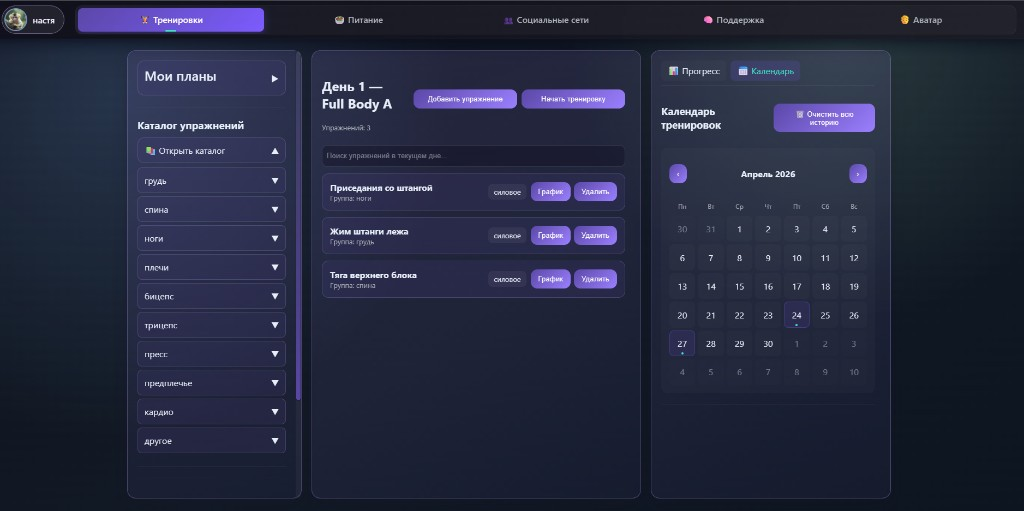
\includegraphics[width=0.92\linewidth]{rp_screen_02.png}
	\caption{Главное окно: модуль тренировок}
	\label{fig:rp-screen-02}
\end{figure}

На рисунке~\ref{fig:rp-screen-03} показано создание или редактирование плана и применение шаблона программы.

\begin{figure}[H]
	\centering
	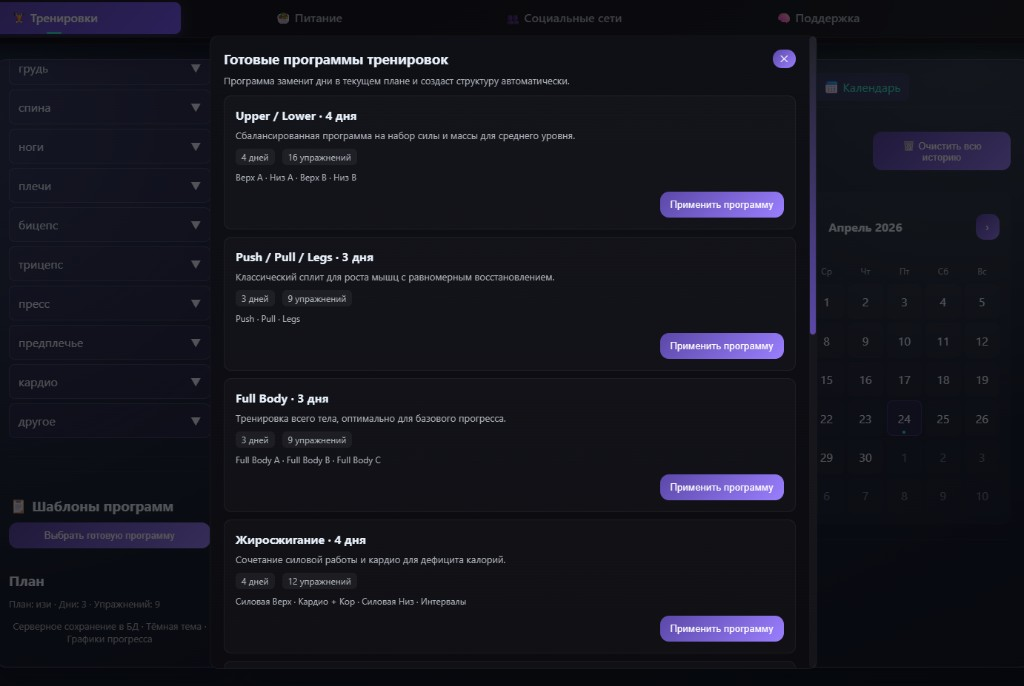
\includegraphics[width=0.92\linewidth]{rp_screen_03.png}
	\caption{Создание тренировочного плана и шаблоны программ}
	\label{fig:rp-screen-03}
\end{figure}

На рисунке~\ref{fig:rp-screen-04} представлен режим выполнения тренировки и фиксация подходов.

\begin{figure}[H]
	\centering
	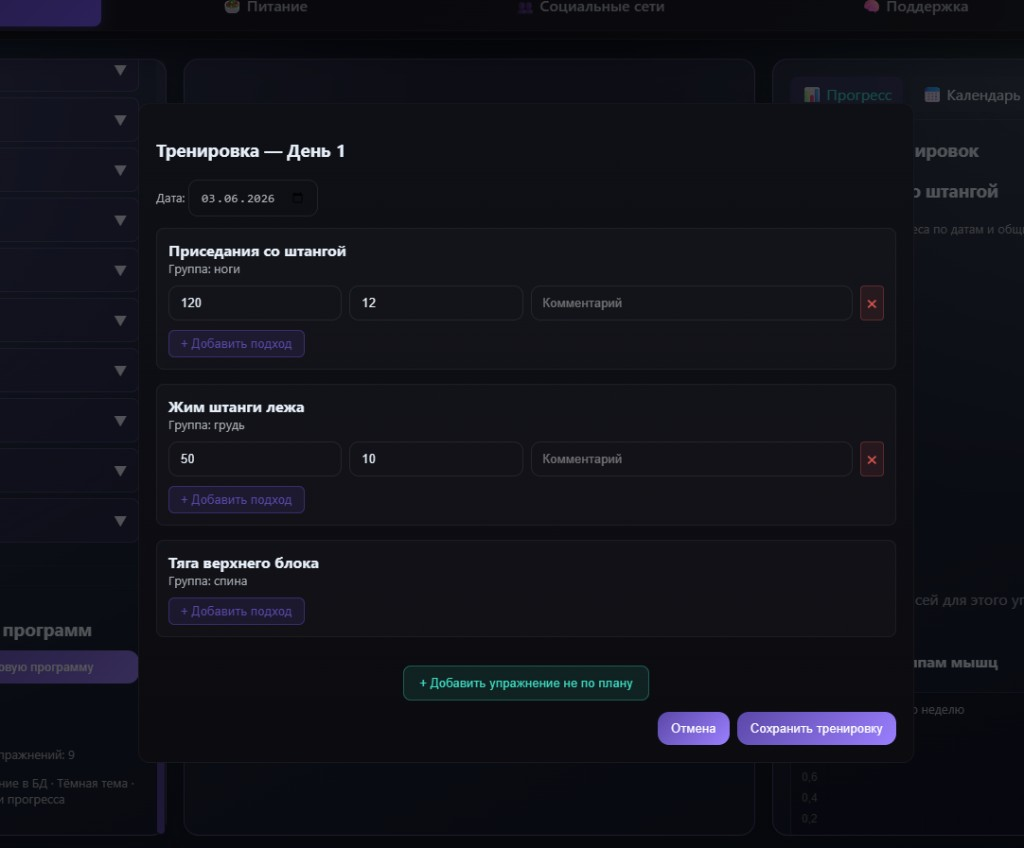
\includegraphics[width=0.92\linewidth]{rp_screen_04.png}
	\caption{Выполнение тренировки по плану}
	\label{fig:rp-screen-04}
\end{figure}

На рисунке~\ref{fig:rp-screen-05} приведены графики прогресса на вкладке <<Прогресс>>.

\begin{figure}[H]
	\centering
	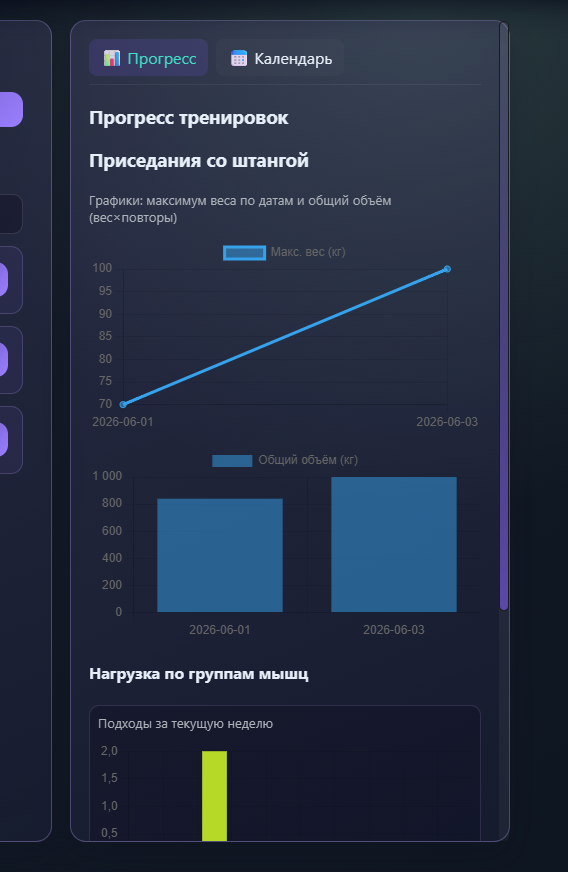
\includegraphics[width=0.92\linewidth]{rp_screen_05.png}
	\caption{Визуализация прогресса и аналитика нагрузки}
	\label{fig:rp-screen-05}
\end{figure}

На рисунке~\ref{fig:rp-screen-06} показан раздел <<Питание>>.

\begin{figure}[H]
	\centering
	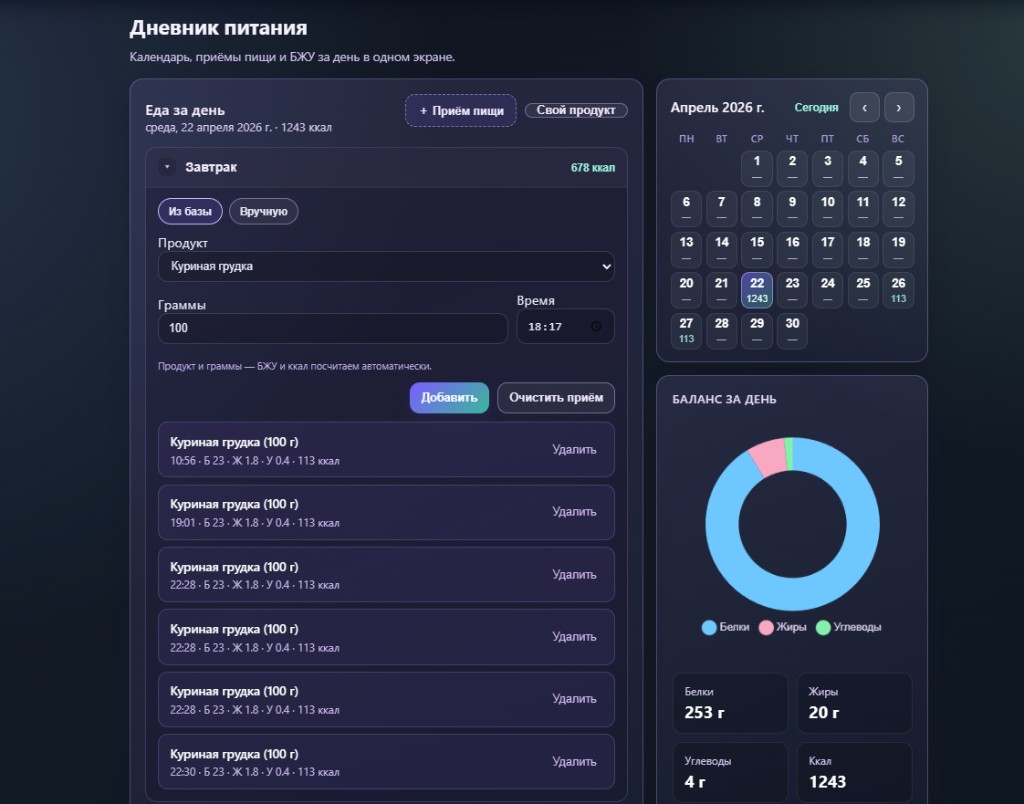
\includegraphics[width=0.92\linewidth]{rp_screen_06.png}
	\caption{Дневник питания и показатели КБЖУ}
	\label{fig:rp-screen-06}
\end{figure}

На рисунке~\ref{fig:rp-screen-07} представлена социальная лента.

\begin{figure}[H]
	\centering
	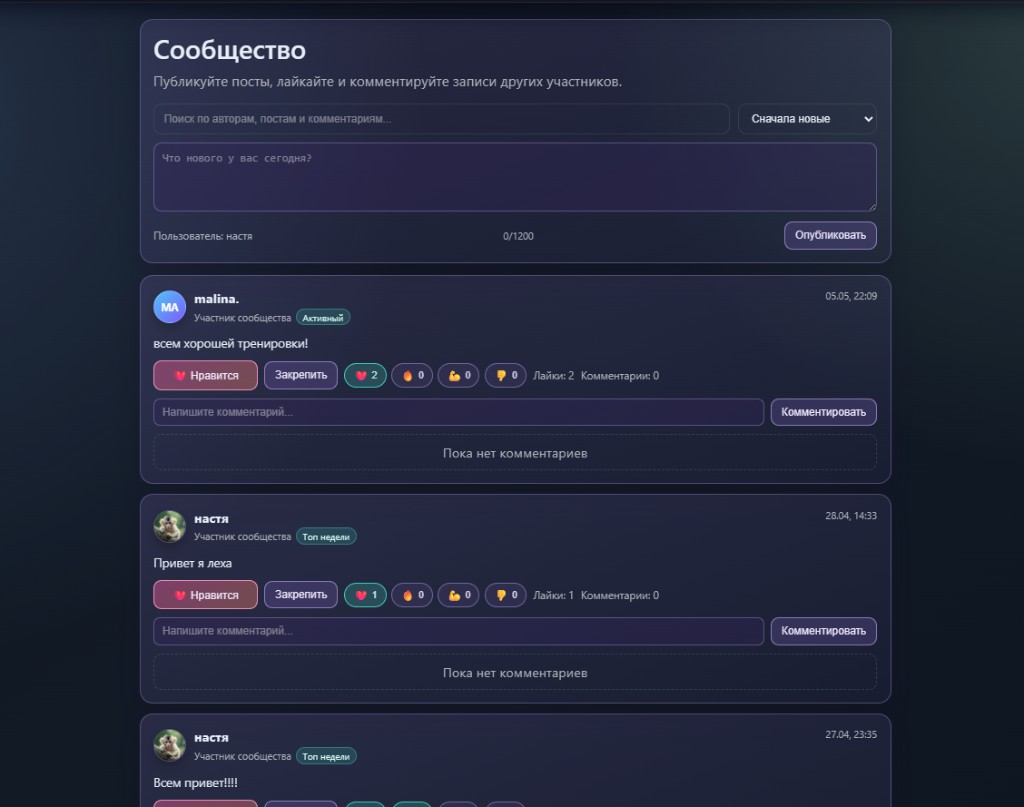
\includegraphics[width=0.92\linewidth]{rp_screen_07.png}
	\caption{Социальная лента и взаимодействие с постами}
	\label{fig:rp-screen-07}
\end{figure}

На рисунке~\ref{fig:rp-screen-08} показан раздел <<Аватар>> с уровнем персонажа и шкалой опыта.

\begin{figure}[H]
	\centering
	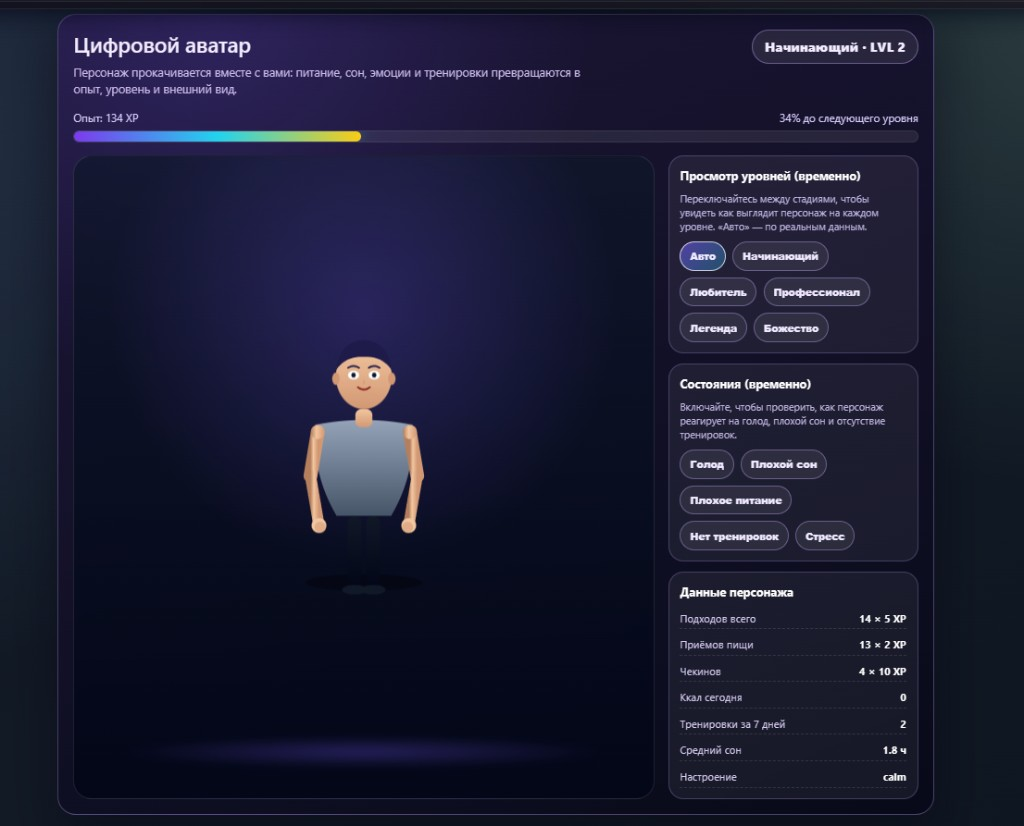
\includegraphics[width=0.92\linewidth]{rp_screen_08.png}
	\caption{Модуль цифрового аватара}
	\label{fig:rp-screen-08}
\end{figure}

На рисунке~\ref{fig:rp-screen-09} представлен профиль пользователя.

\begin{figure}[H]
	\centering
	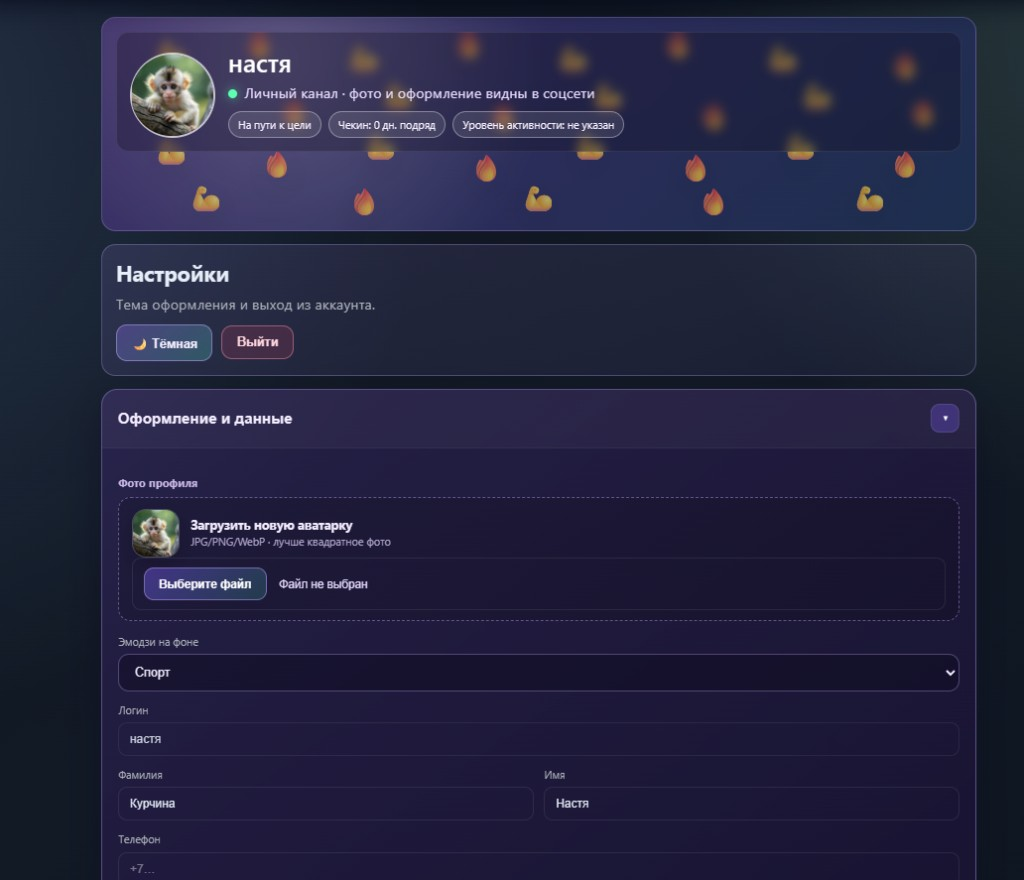
\includegraphics[width=0.92\linewidth]{rp_screen_09.png}
	\caption{Профиль пользователя}
	\label{fig:rp-screen-09}
\end{figure}

На рисунке~\ref{fig:rp-screen-10} показаны модальные окна подтверждения и уведомления.

\begin{figure}[H]
	\centering
	
\includegraphics[width=0.85\linewidth]{rp_screen_10.png}
	\caption{Модальные диалоги приложения}
	\label{fig:rp-screen-10}
\end{figure}

По результатам системного тестирования подтверждено выполнение основных сценариев: регистрация и вход, работа с планами и журналом тренировок, отображение графиков, ведение дневника питания, публикации в социальной ленте, чекины в разделе поддержки, отображение аватара и редактирование профиля. Данные пользователя сохраняются в localStorage и при доступном сервере синхронизируются через API, что позволяет восстановить состояние клиента после перезагрузки страницы.

   \section*{ЗАКЛЮЧЕНИЕ}
\addcontentsline{toc}{section}{ЗАКЛЮЧЕНИЕ}

В выпускной квалификационной работе рассмотрена разработка клиентской подсистемы программно-информационной системы <<Fitness Life>> -- бизнес-проекта стартап-команды, направленного на индивидуальное планирование тренировок, учёт питания и сопутствующую мотивацию пользователя в едином веб-приложении. Выполненный инженерный вклад автора относится к браузерной части продукта: проектированию одностраничного интерфейса, модульной организации клиентского кода и обеспечению взаимодействия с REST API серверной подсистемы, реализуемой напарником по проекту.

В ходе работы изучена предметная область индивидуальных занятий физической культурой, проанализированы аналогичные цифровые сервисы и сформулированы требования к клиентскому приложению. На основе анализа обоснована клиент-серверная архитектура: серверная часть отвечает за аутентификацию, хранение профилей и синхронизируемого пользовательского хранилища, а клиентская -- за представление данных, ввод пользователем и выполнение прикладных сценариев без полной перезагрузки страницы.

Спроектирована и реализована клиентская подсистема в каталоге \texttt{ДИПЛОМ 2} репозитория проекта. Приложение построено как одностраничное веб-приложение (HTML, CSS, JavaScript): единая HTML-страница задаёт каркас экранов авторизации и основной оболочки, модуль \texttt{auth.js} обеспечивает регистрацию, вход, работу с JWT и синхронизацию \texttt{localStorage} с сервером, модуль \texttt{app.js} -- логику тренировочных планов, журнала подходов и визуализации нагрузки с использованием Chart.js. Предметные разделы (профиль, питание, поддержка, социальная лента, аватар) вынесены в отдельные файлы \texttt{*.module.js}, что упрощает сопровождение и развитие функциональности.

Основные результаты работы:
\begin{enumerate}
\item Проведён анализ предметной области и сопоставлены подходы к построению клиентских веб-приложений в сфере фитнеса; определены функциональные требования к клиентской части системы.
\item Разработано техническое задание и технический проект клиентской подсистемы: описаны архитектура одностраничного приложения, состав модулей, работа с DOM, Web Storage API и событийной моделью браузера.
\item Реализованы экраны аутентификации и профиля, клиентские модули тренировок, питания, психологической поддержки, цифрового аватара и социальной ленты.
\item Организовано локальное хранение рабочего состояния пользователя и синхронизация данных с REST API серверной части при наличии сетевого соединения.
\item Выполнено системное тестирование ключевых пользовательских сценариев в браузере: регистрация и вход, работа с планами и журналом тренировок, отображение графиков прогресса, ведение дневника питания, публикации в ленте, чекины в разделе поддержки, отображение аватара и редактирование профиля.
\end{enumerate}

Поставленные во введении и в задании на выпускную квалификационную работу задачи решены. Требования технического задания к клиентской подсистеме выполнены в объёме, необходимом для демонстрации MVP продукта <<Fitness Life>> и согласованной работы с серверной частью. Готовый рабочий проект представлен исходным кодом клиентских модулей, спецификацией методов и результатами проверки интерфейса; фрагменты кода и графический материал приведены в приложениях.

Направления дальнейшего развития клиентской подсистемы включают: замену заглушек скриншотов в разделе тестирования на иллюстрации реального интерфейса; повышение доступности (ARIA, навигация с клавиатуры); оптимизацию загрузки (разбиение на бандлы, ленивая подгрузка модулей); расширение офлайн-режима за счёт Service Worker; углубление аналитики тренировок и интеграцию с носимыми устройствами при развитии серверного API; внедрение элементов freemium-модели монетизации, обозначенной в бизнес-обосновании проекта.

Таким образом, в работе создана работоспособная клиентская часть веб-приложения <<Fitness Life>>, обеспечивающая пользователю единый интерфейс для планирования нагрузки, учёта питания и социально-мотивационных функций с сохранением персональных данных и возможностью их синхронизации между сеансами работы в браузере.

}\fi
\makeatletter
\AtBeginEnvironment{thebibliography}{%
	\section*{\refname}%
	\addcontentsline{toc}{section}{\refname}%
}
\patchcmd{\thebibliography}{\section*{\refname}}{}{}{}
\makeatother
\sloppy

\begin{thebibliography}{99}

    

	\bibitem{ref01}
	Соммервиль~И. Инженерия программного обеспечения / И.~Соммервиль; пер. с англ. \textemdash\ 10-е изд. \textemdash\ Москва : Вильямс, 2019. \textemdash\ 1072~с. \textemdash\ ISBN 978-5-907036-78-5.

	\bibitem{ref02}
	Моргунов~Е.П. PostgreSQL. Основы языка SQL / Е.П.~Моргунов. \textemdash\ Санкт-Петербург : БХВ-Петербург, 2018. \textemdash\ 336~с. \textemdash\ ISBN 978-5-9775-3697-4.

	\bibitem{ref03}
	Выдрин~Д.К., Грибов~А.Ю., Анохин~А.Ю. HTML5 и CSS3. Веб-разработка по стандартам нового поколения / Д.К.~Выдрин, А.Ю.~Грибов, А.Ю.~Анохин. \textemdash\ 2-е изд., перераб. и доп. \textemdash\ Москва : ДМК Пресс, 2021. \textemdash\ 416~с. \textemdash\ ISBN 978-5-97060-957-9.

	\bibitem{ref04_new}
	Робсон~Э., Фримен~Э. Изучаем HTML, XHTML и CSS / Э.~Робсон, Э.~Фримен; пер. с англ. \textemdash\ Санкт-Петербург : Питер, 2009. \textemdash\ 720~с. \textemdash\ ISBN 978-5-388-00622-4.

	\bibitem{ref05}
	Прохоренок~Н.А., Дронов~В.А. JavaScript и Node.js для веб-разработчиков / Н.А.~Прохоренок, В.А.~Дронов. \textemdash\ Санкт-Петербург : БХВ-Петербург, 2022. \textemdash\ 592~с. \textemdash\ ISBN 978-5-9775-6591-9.

	\bibitem{ref06}
	Флэнаган~Д. JavaScript. Подробное руководство / Д.~Флэнаган; пер. с англ. \textemdash\ 7-е изд. \textemdash\ Санкт-Петербург : БХВ-Петербург, 2021. \textemdash\ 1168~с. \textemdash\ ISBN 978-5-9775-4825-9.

	\bibitem{ref07}
	Хавербекке~М. Выразительный JavaScript / М.~Хавербекке; пер. с англ. \textemdash\ 3-е изд. \textemdash\ Санкт-Петербург : Питер, 2022. \textemdash\ 608~с. \textemdash\ ISBN 978-5-4461-1912-3.

	\bibitem{ref09_new}
	Закас~Н. JavaScript для профессиональных веб-разработчиков / Н.~Закас; пер. с англ. \textemdash\ 5-е изд. \textemdash\ Москва : Диалектика, 2020. \textemdash\ 1120~с. \textemdash\ ISBN 978-5-907144-29-9.

	\bibitem{ref12_new}
	Murray~S. Interactive Data Visualization for the Web / S.~Murray. \textemdash\ 3rd ed. \textemdash\ Sebastopol : O'Reilly Media, 2017. \textemdash\ 456~p. \textemdash\ ISBN 978-1491921296.

	\bibitem{ref16_new}
	Фрэйн~Б. Отзывчивый дизайн на HTML5 и CSS3 для любых устройств / Б.~Фрэйн; пер. с англ. \textemdash\ 3-е изд. \textemdash\ Санкт-Петербург : Питер, 2020. \textemdash\ 304~с. \textemdash\ ISBN 978-5-4461-1495-5.

    

	\bibitem{ref17}
	Черников~В.Н. Разработка мобильных приложений на C\# для iOS и Android / В.Н.~Черников. \textemdash\ Москва : ДМК Пресс, 2020. \textemdash\ 188~с. \textemdash\ ISBN 978-5-97060-805-0.

	\bibitem{ref18}
	Льюис~Ш., Данн~М. Нативная разработка мобильных приложений / Ш.~Льюис, М.~Данн; пер. с англ. А.Н.~Киселева. \textemdash\ Москва : ДМК Пресс, 2020. \textemdash\ 376~с. \textemdash\ ISBN 978-5-97060-845-6.

	\bibitem{ref19}
	Браун~И. Веб-разработка с применением Node и Express. Полноценное использование стека JavaScript / И.~Браун; пер. с англ. \textemdash\ 2-е изд. \textemdash\ Санкт-Петербург : Питер, 2022. \textemdash\ 336~с. \textemdash\ ISBN 978-5-4461-0590-8.

	\bibitem{ref20}
	Брэдшоу~Ш., Брэзил~Д., Ходоров~К. Mongo DB: полное руководство / Ш.~Брэдшоу, Д.~Брэзил, К.~Ходоров; пер. с англ. Д.А.~Беликова. \textemdash\ Москва : ДМК Пресс, 2020. \textemdash\ 540~с. \textemdash\ ISBN 978-5-97060-792-3.

	\bibitem{ref21}
	Понуторай~П.К., Лолигер~Дж. Git: контроль версий / П.К.~Понуторай, Дж.~Лолигер. \textemdash\ Астана : Спринт Бук, 2025. \textemdash\ 512~с. \textemdash\ ISBN 978-601-08-4358-5.

	\bibitem{ref22}
	Аниче~М. Эффективное тестирование программного обеспечения / М.~Аниче; пер. с англ. А.Н.~Киселева. \textemdash\ Москва : ДМК Пресс, 2022. \textemdash\ 370~с. \textemdash\ ISBN 978-5-97060-997-2.

	\bibitem{ref23}
	Акулич~М.В. Дизайн пользовательского интерфейса и дизайн UI/UX в разработке мобильных приложений. Базовые знания / М.В.~Акулич. \textemdash\ Москва : ДМК Пресс, 2023. \textemdash\ 180~с. \textemdash\ ISBN 978-5-93700-156-5.

	\bibitem{ref24}
	Рининсланд~Э., Свизек~Т. Визуализация данных с помощью библиотеки D3.js 4.x / Э.~Рининсланд, Т.~Свизек; пер. с англ. А.А.~Слинкина. \textemdash\ 3-е изд. \textemdash\ Москва : ДМК Пресс, 2017. \textemdash\ 298~с. \textemdash\ ISBN 978-5-97060-569-1.

	\bibitem{ref25}
	Макдональд~М. Грокаем безопасность веб-приложений / М.~Макдональд. \textemdash\ Санкт-Петербург : Питер, 2026. \textemdash\ 336~с. \textemdash\ ISBN 978-5-4461-4220-0.

	\bibitem{ref26}
	Коул~Р., Скотчер~Э. Блистательный Agile. Гибкое управление проектами с помощью Agile, Scrum и Kanban / Р.~Коул, Э.~Скотчер. \textemdash\ Санкт-Петербург : Питер, 2019. \textemdash\ 304~с. \textemdash\ ISBN 978-5-4461-1051-3.

	\bibitem{ref27}
	Золкин~А.Л., Айбазов~А.Х., Новикова~Ж.В. и~др. Интеллектуальные системы мониторинга функционального состояния спортсменов на основе комплексных цифровых биомаркеров и машинного обучения : учебник / А.Л.~Золкин, А.Х.~Айбазов, Ж.В.~Новикова. \textemdash\ Москва : Русайнс, 2026. \textemdash\ 198~с. \textemdash\ ISBN 978-5-466-11299-3.

	\bibitem{ref28}
	Костин~А. Нейросети в фитнесе: как тренироваться с ИИ и быстрее видеть результат / А.~Костин. \textemdash\ Электрон. дан. \textemdash\ 2026.

	\bibitem{ref29}
	Орлов~С.А. Программная инженерия. Технологии разработки программного обеспечения : учебник для вузов / С.А.~Орлов. \textemdash\ 5-е изд., обновл. и доп. \textemdash\ Санкт-Петербург : Питер, 2016. \textemdash\ 640~с. \textemdash\ ISBN 978-5-496-01917-0.

	\bibitem{ref30}
	Орлов~С.А. Программная инженерия. Стандарт третьего поколения / С.А.~Орлов. \textemdash\ Санкт-Петербург : Питер, 2020. \textemdash\ 640~с. \textemdash\ ISBN 978-5-4461-1348-4.

	\bibitem{ref31}
	Кочер~П.С. Микросервисы и контейнеры Docker / П.С.~Кочер; пер. с анг. А.Н.~Киселева. \textemdash\ Москва : ДМК Пресс, 2019. \textemdash\ 240~с. \textemdash\ ISBN 978-5-97060-739-8.

	\bibitem{ref32}
	Афанасьев~В.\,В., Осетров~И.\,А., Муравьев~А.\,В., Михайлов~П.\,В. Спортивная метрология : учебник для СПО / В.В.~Афанасьев, И.А.~Осетров, А.В.~Муравьев, П.В.~Михайлов; отв. ред. В.В.~Афанасьев. \textemdash\ 2-е изд., испр. и доп. \textemdash\ Москва : Юрайт, 2022. \textemdash\ 209~с. \textemdash\ (Профессиональное образование). \textemdash\ ISBN 978-5-534-08626-3.

	\bibitem{ref34}
	Петров~П.К. Информационные технологии в физической культуре и спорте : учебник / П.К.~Петров. \textemdash\ Москва : Academia, 2011. \textemdash\ 288~с. \textemdash\ ISBN 978-5-7695-8082-6.

	\bibitem{ref35}
	Молдованова~О.В. Информационные системы и базы данных : учебное пособие для СПО / О.В.~Молдованова. \textemdash\ Саратов : Профобразование, 2022. \textemdash\ 184~с. \textemdash\ ISBN 978-5-4488-1177-7.

	\bibitem{ref36}
	Прокушев~Я.Е. Базы данных : учебник с практикумом / Я.Е.~Прокушев. \textemdash\ 2-е изд. \textemdash\ Санкт-Петербург : Интермедия, 2022. \textemdash\ 264~с. \textemdash\ ISBN 978-5-4383-0250-6.

	\bibitem{ref37}
	Хортон~Дж. Разработка Android-приложений с нуля / Дж.~Хортон; пер. с англ. \textemdash\ 3-е изд. \textemdash\ Санкт-Петербург : БХВ-Петербург, 2023. \textemdash\ 576~с. \textemdash\ ISBN 978-5-9775-6855-5.

	\bibitem{ref38}
	Гриффитс~Д., Гриффитс~Д. Head First. Программирование для Android на Kotlin / Д.~Гриффитс, Д.~Гриффитс; пер. с англ. Е.~Матвеева. \textemdash\ 3-е изд. \textemdash\ Санкт-Петербург : Питер, 2023. \textemdash\ 912~с. \textemdash\ ISBN 978-5-4461-2016-1.

	\bibitem{ref39}
	Лоранс~П.-О., Хинчман-Домингес~А. Программирование на Kotlin для Android / П.-О.~Лоранс, А.~Хинчман-Домингес; пер. с англ. \textemdash\ Санкт-Петербург : БХВ-Петербург, 2024. \textemdash\ 336~с. \textemdash\ ISBN 978-5-9775-0944-2.

	\bibitem{ref41}
	Тидвелл~Дж., Брюэр~Ч., Валенсия~Э. Разработка интерфейсов: паттерны проектирования / Дж.~Тидвелл, Ч.~Брюэр, Э.~Валенсия; пер. с англ. \textemdash\ 3-е изд. \textemdash\ Санкт-Петербург : Питер, 2024. \textemdash\ 555~с. \textemdash\ (Бестселлеры O'Reilly). \textemdash\ ISBN 978-5-4461-1646-1.

	\bibitem{ref42}
	Чернышев~С.А., Петров~Ю.М. Основы Flutter / С.А.~Чернышев, Ю.М.~Петров. \textemdash\ Санкт-Петербург : Питер, 2025. \textemdash\ 688~с. \textemdash\ (Библиотека программиста). \textemdash\ ISBN 978-5-4461-4469-3.

	\bibitem{ref43}
	Мамедли~Р.Э., Казиахмедов~Т.Б. Большие данные и NoSQL базы данных : учебное пособие для СПО / Р.Э.~Мамедли, Т.Б.~Казиахмедов. \textemdash\ 2-е изд., стер. \textemdash\ Санкт-Петербург : Лань, 2026. \textemdash\ 92~с. \textemdash\ ISBN 978-5-507-55047-0.

	\bibitem{ref44}
	Плас~Дж. Вандер. Python для сложных задач: наука о данных / Дж.~Вандер Плас; пер. с англ. Л.~Киселевой. \textemdash\ 2-е изд. \textemdash\ Астана : Спринт Бук, 2025. \textemdash\ 588~с. \textemdash\ (Бестселлеры O'Reilly). \textemdash\ ISBN 978-601-08-3564-1.

\end{thebibliography}

\ifВКР{\appendix{Представление графического материала}

Графический материал, выполненный на отдельных листах,
изображен на рисунках А.1--А.\arabic{числоПлакатов}.
\setcounter{числоПлакатов}{0}

\renewcommand{\thefigure}{А.\arabic{figure}} % шаблон номера для плакатов

\begin{landscape}

\begin{плакат}
    \includegraphics[width=0.82\linewidth]{плакат1.png}
    \заголовок{Сведения о ВКРБ}
    \label{pl1:image}
\end{плакат}

\begin{плакат}
    \includegraphics[width=0.82\linewidth]{плакат2.png}
    \заголовок{Цели и задачи}
    \label{pl2:image}
\end{плакат}

\begin{плакат}
    \includegraphics[width=0.82\linewidth]{плакат3.png}
    \заголовок{Решение проблем}
    \label{pl3:image}
\end{плакат}

\begin{плакат}
    \includegraphics[width=0.82\linewidth]{плакат4.png}
    \заголовок{Диаграмма прецедентов}
    \label{pl4:image}
\end{плакат}

\begin{плакат}
    \includegraphics[width=0.82\linewidth]{плакат5.png}
    \заголовок{Диаграмма компонентов}
    \label{pl5:image}
\end{плакат}

\begin{плакат}
    \includegraphics[width=0.82\linewidth]{плакат6.png}
    \заголовок{Структура основной страницы}
    \label{pl6:image}
\end{плакат}

\begin{плакат}
    \includegraphics[width=0.82\linewidth]{плакат7.png}
    \заголовок{Заключение}
    \label{pl7:image}
\end{плакат}

\end{landscape}
}\fi
\ifПрактика{}\else{\appendix{Фрагменты исходного кода клиентской части}

Ниже приведены фрагменты основных файлов клиентской подсистемы приложения (каталог \texttt{ДИПЛОМ 2}).

\subsection*{213223232.html}

\lstinputlisting[language=Java, frame=none]{code/appendix/213223232-mount.html}

\subsection*{css/styles.css}

\lstinputlisting[language=Java, frame=none, firstline=1, lastline=55]{code/css/styles.css}

\subsection*{js/auth.js}

\lstinputlisting[language=Java, frame=none, firstline=1, lastline=12]{code/js/auth.js}

\lstinputlisting[language=Java, frame=none, firstline=44, lastline=129]{code/js/auth.js}

\lstinputlisting[language=Java, frame=none, firstline=333, lastline=375]{code/js/auth.js}

\subsection*{js/app.js}

\lstinputlisting[language=Java, frame=none, firstline=1, lastline=66]{code/js/app.js}

\lstinputlisting[language=Java, frame=none, firstline=68, lastline=157]{code/js/app.js}

\subsection*{modules/profile.module.js}

\lstinputlisting[language=Java, frame=none, firstline=1, lastline=13]{code/modules/profile.module.js}

\subsection*{modules/nutrition.module.js}

\lstinputlisting[language=Java, frame=none]{code/appendix/nutrition-head.js}

\lstinputlisting[language=Java, frame=none]{code/appendix/nutrition-kcal.js}

\lstinputlisting[language=Java, frame=none]{code/appendix/nutrition-render.js}

\subsection*{modules/avatar.module.js}

\lstinputlisting[language=Java, frame=none, firstline=1, lastline=36]{code/modules/avatar.module.js}

\subsection*{data/mental-advice.json}

\lstinputlisting[language=Java, frame=none]{code/data/mental-advice.json}

\ifВКР{
\newpage
\addcontentsline{toc}{section}{На отдельных листах (CD-RW в прикрепленном конверте)}
\noindent
\begin{tabular}{p{5.8cm}C{4.8cm}C{4.8cm}}
   Автор ВКР & \lhrulefill{\fill} & \fillcenter\Автор \\
            \setarstrut{\footnotesize}
           & \footnotesize{(подпись, дата)} & \\
            \restorearstrut
   Руководитель ВКР & \lhrulefill{\fill} & \fillcenter\Руководитель \\
            \setarstrut{\footnotesize}
           & \footnotesize{(подпись, дата)} & \\
            \restorearstrut
   Нормоконтроль & \lhrulefill{\fill} & \fillcenter\Нормоконтроль \\
            \setarstrut{\footnotesize}
           & \footnotesize{(подпись, дата)} & \\
            \restorearstrut
\end{tabular}
\vskip 2cm
\begin{center}
\textbf{Место для диска}
\end{center}
}\fi
}\fi
\end{document}
